% ÚLTIMA MODIFICACIÓN: 03/01/2024

\documentclass[11pt]{report}

\usepackage{graphicx}
\usepackage[a4paper, right = 0.9in, left = 0.9in, top = 1.3in, bottom = 0.8in]{geometry}
\usepackage[utf8]{inputenc}
\usepackage[spanish]{babel}
\usepackage{amsmath,amsfonts,amssymb,amsthm}
\usepackage{hyperref} % Para poder insertar hiperenlaces a secciones del documento
\usepackage[table, x11names, svgnames]{xcolor} % Para cambiar las letras de color
\usepackage{dirtytalk} % Para usar comillas de apertura y cierre
\usepackage{fbox} % Para las cajas en las demostraciones de "si y solo si" y doble contención
\usepackage{mathtools}
\usepackage{multicol} % Para dividir una lista en varias columnas
\usepackage{soul} % Para cambiar de línea con palabras subrayadas
\usepackage{imakeidx} % Tiene que ver con el índice
\usepackage{graphicx}
\usepackage{faktor} % Conjuntos cociente
\usepackage{float} % Para que algunas figuras no se coloquen al inicio de la página
\usepackage{centernot} % Para negar símbolos como \implies
\usepackage{spalign}
\usepackage{array}
\usepackage[outline]{contour}
\usepackage{ulem}
\usepackage{color}
\usepackage{fancyhdr}
\usepackage[framemethod=tikz]{mdframed}
\usepackage{bm}
\usetikzlibrary{shadows} % Sombras de los recuadros
\usepackage{setspace} % Espacio entre líneas del índice
\usepackage{pgfplots}
\usepgfplotslibrary{fillbetween}
\usepackage{tikz}
\usepackage{tikz-cd}
\usetikzlibrary{patterns}
\usetikzlibrary{cd} % Diagramas conmutativos
\usepackage{bbm} % Usar \mathbb con símbolos matemáticos
\usepackage{pdfpages}

\newenvironment{cdefinition} % Maniobras para meter una definición en un recuadro
  {\begin{mdframed}[innertopmargin = 0pt,
                    innerbottommargin = 7.5pt,
                    backgroundcolor = lightgray!10,
                    linewidth = 1pt,
                    shadow = true,
                    shadowsize = 5pt,
                    roundcorner = 0pt,
                    skipabove = 0pt]
    \begin{definition}}
  {\end{definition}\end{mdframed}}

\newenvironment{ctheorem} % Maniobras para meter un teorema en un recuadro
  {\begin{mdframed}[innertopmargin = 0pt,
                    innerbottommargin = 7.5pt,
                    backgroundcolor = lightgray!10,
                    linewidth = 1pt,
                    shadow = true,
                    shadowsize = 5pt,
                    roundcorner = 0pt,
                    skipabove = 0pt]
    \begin{theorem}}
  {\end{theorem}\end{mdframed}}

\newenvironment{cproposition} % Maniobras para meter una proposición en un recuadro
  {\begin{mdframed}[innertopmargin = 0pt,
                    innerbottommargin = 7.5pt,
                    backgroundcolor = lightgray!10,
                    linewidth = 1pt,
                    shadow = true,
                    shadowsize = 5pt,
                    roundcorner = 0pt,
                    skipabove = 0pt]
    \begin{proposition}}
  {\end{proposition}\end{mdframed}}

\newenvironment{ccorollary} % Maniobras para meter un corolario en un recuadro
  {\begin{mdframed}[innertopmargin = 0pt,
                    innerbottommargin = 7.5pt,
                    backgroundcolor = lightgray!10,
                    linewidth = 1pt,
                    shadow = true,
                    shadowsize = 5pt,
                    roundcorner = 0pt,
                    skipabove = 0pt]
    \begin{corollary}}
  {\end{corollary}\end{mdframed}}

\makeatletter % Maniobras para que el subrayado respete las partes de abajo de las letras largas (ahora mismo no lo uso)
\newcommand*{\whiten}[1]{\llap{\textcolor{white}{{\the\SOUL@token}}\hspace{#1pt}}}
\DeclareRobustCommand*\sub{%
    \def\SOUL@everyspace{\underline{\space}\kern\z@}%
    \def\SOUL@everytoken{%
     \setbox0=\hbox{\the\SOUL@token}%
     \ifdim\dp0>\z@
        \raisebox{\dp0}{\underline{\phantom{\the\SOUL@token}}}%
        \whiten{1}\whiten{0}%
        \whiten{-1}\whiten{-2}%
        \llap{\the\SOUL@token}%
     \else
        \underline{\the\SOUL@token}%
     \fi}%
\SOUL@}
\makeatother

\makeindex[columns=3, intoc]

\setlength{\columnsep}{0.8cm} % Recta que separa dos columnas (multicols)
\setlength{\columnseprule}{1.5pt}

\makeatletter % Para que el título de los teoremas estén en negrita
\def\th@plain{%
  \thm@notefont{}
  \itshape
}
\def\th@definition{
  \thm@notefont{}
  \normalfont
}
\makeatother

\graphicspath{{./images/}}

\newtheorem{proposition}{Proposición}[chapter]
\newtheorem{corollary}{Corolario}[chapter]
\newtheorem{theorem}{Teorema}[chapter]
\newtheorem*{theorem*}{Teorema} % Teoremas especiales sin numerar
\theoremstyle{definition}
\newtheorem{definition}{Definición}[chapter]
\theoremstyle{definition}
\newtheorem{example}{Ejemplo}[chapter]
\theoremstyle{remark}
\newtheorem*{obs}{Observación} % * para que no se numeren
\renewcommand*{\proofname}{Demostración}
\addto\captionsspanish{\renewcommand{\chaptername}{Tema}} % Para que ponga "Tema 1" en vez de "Capítulo 1"
\addto\captionsspanish{\renewcommand{\contentsname}{Índice}} % Para cambiar el título del índice

\setuldepth{Berlin}

\newcommand*{\Scale}[2][4]{\scalebox{#1}{$#2$}}%

% Shortcuts:
\newcommand{\R}{\mathbb R}
\newcommand{\N}{\mathbb N}
\newcommand{\Z}{\mathbb Z}
\newcommand{\Q}{\mathbb Q}
\newcommand{\C}{\mathbb C}

%--------------------------------------------------------------------------------------------------%

% CAMBIAR EL SÍMBOLO \in POR EL DEL PAQUETE mathabx; IMPORTAR \bigast

\DeclareFontFamily{U}{matha}{}
\DeclareFontShape{U}{matha}{m}{n}{
  <-5.5> matha5
  <5.5-6.5> matha6
  <6.5-7.5> matha7
  <7.5-8.5> matha8
  <8.5-9.5> matha9
  <9.5-11> matha10
  <11-> matha12
}{}
\DeclareSymbolFont{matha}{U}{matha}{m}{n}
\DeclareFontSubstitution{U}{matha}{m}{n}
\DeclareMathSymbol{\in}{3}{matha}{"50}

\DeclareFontFamily{U}{mathb}{}
\DeclareFontShape{U}{mathb}{m}{n}{
  <-5.5> mathb5
  <5.5-6.5> mathb6
  <6.5-7.5> mathb7
  <7.5-8.5> mathb8
  <8.5-9.5> mathb9
  <9.5-11> mathb10
  <11-> mathb12
}{}
\DeclareSymbolFont{mathb}{U}{mathb}{m}{n}
\DeclareFontSubstitution{U}{mathb}{m}{n}
\DeclareMathSymbol{\bigast}{1}{mathb}{"06}

%--------------------------------------------------------------------------------------------------%

\begin{document}

% Longitud antes y después de una expresión matemática:
\setlength{\abovedisplayskip}{10pt}
\setlength{\belowdisplayskip}{10pt} % Ocultar el contador de páginas pero seguir contando

\pagestyle{empty}

\begin{center}
    \vspace*{1cm} % Sin el asterisco, \vspace se ignora al principio del documento
    \Huge \textbf{Topología Algebraica Básica}
        
    \vspace{10mm} % \vspace tiene que estar separado de la línea anterior para que funcione
    \large
%    David López
        
%    \vspace{5mm}
\textit{Universidad de Málaga \\[5pt]
Grado en Matemáticas \\[5pt]
Curso 2023-2024}
\end{center}

\doublespacing
\tableofcontents
\singlespacing

\pagestyle{fancy}
\renewcommand{\chaptermark}[1]{\markboth{#1}{}}
\fancyhf{}
\fancyhead[R]{\textbf{\scriptsize \thepage}}
\fancyhead[L]{\textbf{\scriptsize \chaptername \ \thechapter. \leftmark}}

\fancypagestyle{plain}{%
\fancyhead{}
\fancyfoot{}
\renewcommand{\footrulewidth}{0pt} 
\renewcommand{\headrulewidth}{0pt}
}

\chapter{Homotopía}

\section{Nociones básicas}
De aquí en adelante, las aplicaciones entre espacios topológicos que aparezcan se supondrán continuas (a veces se escribirá y a veces no). Además, se entenderá que $I = [0,1]$ para ahorrar escritura.

\hfill

\begin{cdefinition}
Sean $f,g \colon X \to Y$ dos aplicaciones continuas entre espacios topológicos $X$ e $Y$. Se dice que \textbf{\textit{$\bm{f}$ es homótopa a $\bm{g}$}}, y se denota $f \simeq g$, si existe una aplicación continua $H \colon X \times I \to Y$ tal que $H(x,0) = f(x)$ y $H(x,1) = g(x)$ para todo $x \in X$. En tal caso, a $H$ se le denomina \textbf{\textit{homotopía entre $\bm{f}$ y $\bm{g}$}}, y habitualmente se escribe $H \colon f \simeq g$.
\end{cdefinition}

\begin{cdefinition}
    Sean $f, g \colon X \to Y$ dos aplicaciones continuas entre espacios topológicos $X$ e $Y$. Sea $X_0 \subset X$ tal que $f|_{X_0} = g|_{X_0}$. Se dice que \textbf{\textit{$\bm{f}$ es homótopa a $\bm{g}$ relativa a $\bm{X_0}$}}, y se denota $f \simeq_{X_0} g$, si existe una aplicación continua $H \colon X \times I \to Y$ tal que 
    \begin{itemize}
        \item[\textit{(i)}] $H(x,0) = f(x)$ y $H(x,1) = g(x)$ para todo $x \in X$.
        \item[\textit{(ii)}] $H(x_0,t) = f(x_0) = g(x_0)$ para todo $x_0 \in X_0$ y todo $t \in I$.
    \end{itemize}
    En tal caso, a $H$ se le denomina \textbf{\textit{homotopía relativa a $\bm{X_0}$ entre $\bm{f}$ y $\bm{g}$}}, y habitualmente se escribe $H \colon f \simeq_{X_0} g$.
\end{cdefinition}

\begin{example}
    Sean $X = Y = \R^n$ y considérense las aplicaciones
\[
\begin{aligned}[t]
    id \colon \R^n &\longrightarrow \R^n \\
    x &\longmapsto x
\end{aligned}
\qquad
\begin{aligned}[t]
    c_0 \colon \R^n &\longrightarrow \R^n \\
    x &\longmapsto 0
\end{aligned}
\]
Se va a probar que $id \simeq c_0$. Se define la aplicación
\[
\begin{aligned}[t]
    H \colon \R^n \times I &\longrightarrow \R^n \\
    (x,t) &\longmapsto (1-t)x,
\end{aligned}
\]
que es continua y verifica $H(x,0) = x = id(x)$ y $H(x,1) = 0 = c_0(x)$. Por tanto, $H \colon id \simeq c_0$. Es más, como $H(0,t) = 0$ para todo $t \in I$, entonces $H \colon id \simeq_{\{0\}} c_0$.
\end{example}

\begin{example}
    Sean $X = Y = B(0;1) \subset \R^2$ (se utilizará la notación $D^2 = B(0;1)$. Considérense las aplicaciones
\[
\begin{aligned}[t]
    f \colon D^2 &\longrightarrow D^2 \\
    x &\longmapsto x
\end{aligned}
\qquad
\begin{aligned}[t]
    g \colon D^2 &\longrightarrow D^2 \\
    x &\longmapsto -x
\end{aligned}
\]
Se va a probar que $f \simeq g$. Se define la aplicación
\[
\begin{aligned}[t]
    H \colon D^2 \times I &\longrightarrow D^2 \\
    (x,t) &\longmapsto (1-t)f(x)+tg(x)
\end{aligned}
\]
Es importante verificar que $H$ está bien definida, es decir que $H(D^2 \times I) \subset D^2$. En efecto, si $x \in D^2$ y $t \in I$, se tiene que $||(1-2t)x|| = |1-2t| \, ||x|| \leq 1$, luego $H(x,t) = (1-2t)x \in D^2$. Habiéndose quedado uno tranquilo, se puede observar que $H$ es continua y verifica $H(x,0)= x= f(x)$ y $H(x,1) = -x = g(x)$. Por tanto, $H \colon f \simeq g$. Es más, como $H(0,t) = 0$ para todo $t \in I$, entonces $H \colon f \simeq_{\{0\}} g$. 
\end{example}

\begin{example}
Se va a construir otra homotopía entre las aplicaciones del ejemplo anterior, y va a ser la siguiente:
\[
\begin{aligned}[t]
    F \colon D^2 \times I &\longrightarrow D^2 \\
    ((x,y),t) &\longmapsto \begin{pmatrix*}[r]
        \cos \pi t & -\sen \pi t \\
        \sen \pi t & \cos \pi t
    \end{pmatrix*} \begin{pmatrix*}
        x \\
        y
    \end{pmatrix*}
\end{aligned}
\]
En efecto, $F$ es evidentemente continua y además se tiene que $F((x,y),0) = (x,y) = f(x,y)$ y también $F((x,y),1) = (-x,-y) = g(x,y)$. Por tanto, $F \colon f \simeq g$. Al igual que en los otros ejemplos, es claro que $F \colon f \simeq_{\{0\}} g$.
\end{example}

\begin{ctheorem}
La relación de homotopía es una relación de equivalencia en el conjunto de aplicaciones continuas entre dos espacios topológicos $X \!$ e $Y$.
\end{ctheorem}

\begin{proof}
\hfill
\begin{itemize}
    \item[\textit{(i)}] Sea $f \colon X \to Y$ una aplicación entre espacios topológicos. Para ver que $f \simeq f$ solo hay que tomar la aplicación $H \colon X \times I \to Y$ definida por $H(x,t) = f(x)$.
    \item[\textit{(ii)}] Sean $f,g \colon X \to Y$ tales que $f \simeq g$. Esto significa que existe una aplicación $H \colon X \times I \to Y$ tal que $H(x,0) = f(x)$ y $H(x,1) = g(x)$. Se define $F \colon X \times I \to Y$ mediante $F(x,t) = H(x,1-t)$ y una simple comprobación demuestra que $g \simeq f$.
    \item[\textit{(iii)}] Sean $f,g,h \colon X \to Y$ y supóngase que $f \simeq g$ y $g \simeq h$, esto es, que existen aplicaciones $F,G \colon X \times I \to Y$ tales que $F(x,0) = f(x), F(x,1) = g(x), G(x,0) = g(x)$ y $G(x,1) = h(x)$. Se define la aplicación $H \colon X \times I \to Y$ mediante
    \[H(x,t) = \begin{cases}
        F(x,2t) & $si$ \ 0 \leq t \leq \frac{1}{2} \\
        G(x,2t-1) & $si$ \ \frac{1}{2} \leq t \leq 1
    \end{cases}\]
    La función definida por $F(x,2t)$ es continua en el cerrado $X \times [0,\frac{1}{2}]$, mientras que la función definida por $G(x,2t-1)$ es continua en el cerrado $X \times [\frac{1}{2},1]$. Como ambos cerrados recubren $X \times I$ y en la intersección de los cerrados las imágenes coinciden, entonces puede afirmarse que $H$ es continua. Como además $H(x,0) = F(x,0) = f(x)$ y $H(x,1) = G(x,1) = h(x)$, entonces $f \simeq h$.
\end{itemize}
Habiendo comprobado que se verifican las propiedades reflexiva, simétrica y transitiva, no queda nada que demostrar.
\end{proof}

\begin{theorem}
La relación de homotopía relativa a un subespacio es una relación de equivalencia en el conjunto de aplicaciones continuas entre dos espacios topológicos $X \!$ e $Y$ que coinciden en dicho subespacio.
\end{theorem}

\begin{proof}
    Extremadamente similar a la anterior.
\end{proof}

\begin{definition}
    Sea $f \colon X \to Y$ una aplicación continua entre espacios topológicos. 
    \begin{itemize}
        \item[\textit{(i)}] A la clase de equivalencia $f$ en la relación de homotopía, denotada por $[f]$, se le llama \textbf{\textit{clase de homotopía de $\bm{f}$}}.
        \item[\textit{(ii)}] A la clase de equivalencia $f$ en la relación de homotopía relativa a un subespacio $X_0 \subset X$, denotada por $[f]_{X_0}$, se le llama \textbf{\textit{clase de homotopía de $\bm{f}$ relativa a $\bm{X_0}$}}.
    \end{itemize}
    El conjunto cociente será denotado por $[X,Y]$.
\end{definition}

\begin{theorem}
\label{teo1.3.}
    Las composiciones de aplicaciones homótopas resultan aplicaciones homótopas.
\end{theorem}

\begin{proof}
Dados tres espacios topológicos $X,Y$ y $Z$, el panorama es el siguiente:
\[X \xrightarrow{f_1, \, g_1} Y \xrightarrow{f_2, \, g_2} Z, \qquad \qquad f_1 \simeq g_1, \qquad \qquad f_2 \simeq g_2,\]
y hay que demostrar que $f_2 \circ f_1 \simeq g_2 \circ g_1$.

\vspace{2mm}

Como $f_1 \simeq_{X_0} g_1$, existe $F \colon X \times I \to Y$ continua tal que $F(x,0) = f_1(x), F(x,1) = g_1(x)$ y $F(x_0,t)=f_1(x_0)=g_1(x_0)$ para todos los $x, x_0, t$ que estén donde tienen que estar. Y como $f_2 \simeq_{Y_0} g_2$, existe una aplicación $G \colon Y \times I \to Z$ continua tal que $G(y,0) = f_2(y), G(y,1) = g_2(y)$ y $G(y_0,t)=f_2(y_0)=g_2(y_0)$ para todos los $y, y_0, t$ que estén donde tienen que estar.

\vspace{2mm}

Ahora se va a considerar la aplicación $g_2 \circ F \colon X \times I \to Z$, que es evidentemente continua. Se verifica que 
\begin{itemize}
    \item[\textit{(i)}] $g_2 \circ F (x,0) = g_2 \circ f_1 (x)$;
    \item[\textit{(ii)}] $g_2 \circ F (x,1) = g_2 \circ g_1 (x)$.
\end{itemize}

Se ha probado que $g_2 \circ f_1 \simeq g_2 \circ g_1$. Análogamente, se considera la también continua aplicación $G \circ (f_1 \times id_I) \colon X \times I \to Z$, verificando
\begin{itemize}
    \item[\textit{(i)}] $G \circ (f_1 \times id_I) (x,0) = G(f_1(x),0) = f_2 \circ f_1 (x)$;
    \item[\textit{(ii)}] $G \circ (f_1 \times id_I) (x,1) = G(f_1(x),1) = g_2 \circ f_1 (x)$.
\end{itemize}

Ahora se ha probado que $f_2 \circ f_1 \simeq g_2 \circ f_1$, y la transitividad de la relación de homotopía permite afirmar que $f_1 \circ f_2 \simeq g_2 \circ g_1$.
\end{proof}

\begin{theorem}
    Las composiciones de aplicaciones homótopas relativas a un subespacio resultan aplicaciones homótopas relativas al mismo subespacio.
\end{theorem}

\begin{proof}
Extremadamente similar a la anterior.
\end{proof}

\begin{cdefinition}
Dos espacios topológicos $X$ e $Y$ se dice que \textbf{\textit{son homótopos}} o que \textbf{\textit{tienen el mismo tipo de homotopía}} si existen aplicaciones continuas $f \colon X \to Y$ y $g \colon Y \to X$ tales que $g \circ f \simeq id_X$ y $f \circ g \simeq id_Y$. En tal caso, se escribe $X \simeq Y$, y se dice que $f$ y $g$ son \textbf{\textit{equivalencias de homotopía}}.
\end{cdefinition}

Es fácil demostrar que \textit{ser homótopos} o \textit{tener el mismo tipo de homotopía} es una relación de equivalencia. Además, si dos espacios $X$ e $Y$ son homeomorfos, entonces tienen el mismo tipo de homotopía. Sin embargo, como se verá con más detalle próximamente, el recíproco no es cierto. 

\vspace{2mm}

Por último, existen invariantes topológicos que no son invariantes homotópicos. Por ejemplo, $\R^n$ no es compacto y un punto sí, a pesar de tener el mismo tipo de homotopía (como se va a probar en la sección que sigue).

\section{Espacios contráctiles}

El espacio topológico constituido por un solo punto aparecerá con frecuencia en esta sección, y se usará la notación $\{\ast\}$ o simplemente $\ast$ para referirse a él. 

\vspace{2mm}

También será útil remarcar que a las aplicaciones entre espacios topológicos $X$ e $Y$ que envían todos los puntos de $X$ a $y_0 \in Y$ se les denotará por $c_{y_0}^X$, o simplemente $c_{y_0}$ cuando no quepa duda.

\hfill

\begin{cdefinition}
    Un espacio topológico $X$ es \textbf{\textit{contráctil}} si tiene el mismo tipo de homotopía que el espacio formado por un solo punto.
\end{cdefinition}

\begin{proposition}
    Un espacio topológico $X$ es contráctil si y solo si $id_X \simeq c_{x_0}$ para cierto $x_0 \in X$.
\end{proposition}

\begin{proof} Si $X$ es contráctil, existen aplicaciones $f \colon X \to \{\ast\}$ y $g \colon \{\ast\} \to X$ de manera que $g \circ f \simeq id_X$ y $f \circ g \simeq id_{\{\ast\}}$. Como $f = c_\ast$ y $g$ viene dada por $g(\ast) = x_0$ para algún $x_0 \in X$, entonces $g \circ f = c_{x_0} \simeq id_X$.

\vspace{2mm}

Recíprocamente, si $id_X \simeq c_{x_0}$ para cierto $x_0 \in X$, hay que encontrar $f \colon X \to \{\ast\}$ y $g \colon \{\star\} \to X$ tales que $g \circ f \simeq id_X$ y $f \circ g \simeq id_{\{\ast\}}$. Naturalmente, se va a escoger $f = c_\ast$ y $g$ la aplicación definida por $g(\ast) = x_0$, pues en este caso se tiene $g \circ f = c_{x_0} \simeq id_X$ y $f \circ g = id_\ast$, de donde se deduce que $X \simeq \{\ast\}$.
\end{proof}

\begin{proposition}
    Sea $f \colon Y \to X$ una aplicación continua entre espacios topológicos. Si $X$ es contráctil, entonces $f \simeq c_{x_0}^Y$, donde el punto $x_0 \in X$ es el que brinda la proposición anterior.
\end{proposition}

\begin{proof}
Teniendo en cuenta que $id_X \simeq c_{x_0}^X$ por ser $X$ contráctil y haciendo uso del \hyperref[teo1.3.]{\color{blue}Teorema 1.3}, la demostración es tan simple como afirmar $f = id_X \circ f \simeq c_{x_0}^X \circ f = c_{x_0}^Y$.
\end{proof}

\begin{corollary}
    Si $X$ es un espacio topológico contráctil, entonces $id_X \simeq c_x$ para todo $x \in X$.
\end{corollary}

\begin{proof}
    No hay más que aplicar la proposición anterior con $f = c_x$.
\end{proof}

\begin{example}
$\R^n$ es contráctil. En efecto, tomando la aplicación $H \colon \R^n \times I \to \R^n$ definida por $H(x,t) = tx$ se comprueba inmediatamente que $id_{\R^n} \simeq c_{\{0\}}$.
\end{example}

Para el siguiente ejemplo convendría recordar que un subespacio $X \subset \R^n$ es \textit{estrellado respecto de un punto $x_0 \in X$} si el segmento $\overline{x_0x} = \{(1-t)x+tx_0 \colon t \in [0,1]\}$ está contenido en $X$ para todo $x \in X$.

\begin{example}
Cualquier subespacio $X \subset \R^n$ estrellado es contráctil. En efecto, no hay más que tomar la aplicación $H \times X \to I \to X$ definida por $H(x,t) = (1-t)x+tx_0$ (nótese que está bien definida porque $H(X \times I) \subset X$ al ser $X$ estrellado). Se tiene que $H$ es continua y verifica $H(x,0) = x = id_X(x)$ y $H(x,1) = x_0 = c_{x_0}(x)$, lo que demuestra $id_X \simeq c_{x_0}$.
\end{example}

\begin{example}
Existen espacios contráctiles que no son estrellados respecto de ninguno de sus puntos, como por ejemplo $S^n \setminus \{\ast\}$. En efecto, $S^n \setminus \{\ast\}$ es contráctil porque $S^n \setminus \{\ast\} \cong \R^n \simeq \{\ast\}$ y por tanto $S^n \setminus \{\ast\} \simeq \{\ast\}$.
\end{example}

\section{Aplicaciones homotópicamente triviales}

\begin{cdefinition}
Dados dos espacios topológicos $X$ e $Y$, una aplicación continua $f \colon X \to Y$ es \textbf{\textit{homotópicamente trivial}} si $f \simeq c_{y_0}$ para algún $y_0 \in Y$.
\end{cdefinition}

\begin{proposition}
Una aplicación es homotópicamente trivial si y solo si factoriza salvo homotopía por un espacio contráctil.
\end{proposition}
\begin{proof}
Antes que nada, lo de que $f$ \textit{factoriza salvo homotopía por un espacio contráctil} quiere decir que existen aplicaciones continuas $g \colon X \to Z$ y $h \colon Z \to Y$ tales que $f \simeq h \circ g$, siendo $Z$ un espacio topológico contráctil.

\vspace{2mm}

Supóngase entonces que $f \simeq c_{y_0}$ para algún $y_0 \in Y$, siendo $f \colon X \to Y$ continua. Basta tomar las aplicaciones
\[
\begin{aligned}[t]
    c_\ast \colon X &\longrightarrow \{\ast\} \\
    x &\longmapsto \ast
\end{aligned} \qquad \qquad
\begin{aligned}[t]
    y_0 \colon \{\ast\} &\longrightarrow Y \\
    \ast &\longmapsto y_0
\end{aligned}
\]
Se tiene entonces que $f \simeq c_{y_0} = y_0 \circ c_\ast$.

\vspace{2mm}

Supóngase ahora que existen aplicaciones $g \colon X \to Z$ y $h \colon Z \to Y$ con $Z$ contráctil tales que $f \simeq h \circ g$. Se tiene que $h \circ g = h \circ id_Z \circ g \simeq h \circ c_{z_0} \circ g = c_{h(z_0)}$ para cierto $z_0 \in Z$. Como $f \simeq c_{h(z_0)}$, entonces es homotópicamente trivial.
\end{proof}

Conviene recordar para la proposición siguiente que la \textit{esfera unidad de $\R^{n+1}$} es el subespacio $S^n = \{x \in \R^{n+1} \colon ||x|| = 1\}$, y el \textit{disco unidad de $\R^{n+1}$} es $D^{n+1} = \{x \in \R^{n+1} \colon ||x||\leq 1\}$.

\begin{proposition}
\label{prop1.4.}
Sea $Y$ un espacio topológico y sea $f \colon S^n \to Y$ una aplicación continua. Entonces $f$ se extiende a $D^{n+1}$ si y solo si $f$ es homotópicamente trivial.
\end{proposition}

\begin{proof}
Que $f$ \textit{se extiende al disco unidad} quiere decir que existe $\Tilde{f} \colon D^{n+1} \to Y$ continua tal que $\Tilde{f} |_{S^n} = f$. 

\vspace{2mm}

Supóngase primero que $f$ se extienda al disco. Como $D^{n+1} \simeq \{\ast\}$, entonces $f$ factoriza por un espacio contráctil, y por la proposición anterior, $f$ es homotópicamente trivial.

\vspace{2mm}

Si $f$ es homotópicamente trivial, entonces existe $H \colon S^n \times I \to Y$ tal que $H(x,0) = f(x)$ y $H(x,1) = y_0$, para todo $x \in S^n$ y para cierto $y_0 \in Y$. Se define la aplicación $\Tilde{f} \colon D^{n+1} \to Y$ mediante

\[\Tilde{f}(x) = \begin{cases}
        y_0 & $si$ \ 0 \leq ||x|| \leq \frac{1}{2} \\
        H\Bigl(\frac{x}{||x||}, 2-2||x||\Bigr) & $si$ \ \frac{1}{2} \leq ||x|| \leq 1
\end{cases}\]

Nótese que la funciones de cada trozo son continuas y están bien definidas. La intersección de los trozos (que son cerrados que recubren $D^{n+1}$) es $\{x \in D^{n+1} \colon ||x|| = \frac{1}{2}\}$, en cuyo caso las posibles imágenes por $\Tilde{f}$ serían $y_0$ y $H(2x, 2-1) = H(2x,1) = y_0$. Se puede concluir entonces que $\Tilde{f}$ es continua. Además, si $x \in S^n$, entonces $\Tilde{f}(x) = H(x,0) = f(x)$, luego $\Tilde{f}$ extiende a $f$.
\end{proof}

\section{Un invariante algebraico del tipo de homotopía de espacios topológicos}

Cabe destacar que en esta sección podrían sustituirse las palabras "<componentes arcoconexas"> por "<componentes conexas"> y no pasaría absolutamente nada.

\vspace{2mm}

Sea $X$ un espacio topológico. Se denotará por $\pi_0(X)$ al conjunto de componentes arcoconexas de $X$. Dada una aplicación continua $f \colon X \to Y$, se define la aplicación $\pi_0(f) \colon \pi_0(X) \to \pi_0(Y)$ mediante $\pi_0(f)(C) = D$, siendo $D$ la única componente arcoconexa de $Y$ que contiene a $f(C)$. Es fácil demostrar que $\pi_0(id_X) = id_{\pi_0(X)}$ y que $\pi_0(g \circ f) = \pi_0(g) \circ \pi_0(f)$, siendo $f \colon X \to Y$ y $g \colon Y \to Z$ aplicaciones continuas. Estamos entonces en condiciones de enunciar el teorema que protagoniza esta sección.

\hfill

\begin{ctheorem}
    Si $X$ e $Y$ son espacios topológicos con el mismo tipo de homotopía, entonces los conjuntos $\pi_0(X)$ y $\pi_0(Y)$ tienen el mismo cardinal.
\end{ctheorem}

\begin{proof}
Primero se va a demostrar que dos aplicaciones $f,g \colon X \to Y$ homótopas verifican $\pi_0(f) = \pi_0(g)$. 

\vspace{2mm}

Sea $C$ una componente arcoconexa de $X$ y sea $H \colon X \times I \to Y$ la homotopía entre $f$ y $g$. Llámese $D$ a la única componente arcoconexa que contiene a $H(C \times I)$ (es la única porque $H$ es continua y $C \times I$ es producto de subespacios arcoconexos). Se tiene que $f(C) = H(C \times \{0\}) \subset H(C \times I) \subset D$ y también $g(C) = H(C \times \{1\}) \subset H(C \times I) \subset D$, por lo que $\pi_0(f)(C) = D = \pi_0(g)(C)$. Esto prueba que $\pi_0(f) = \pi_0(g)$.

\vspace{2mm}

Supóngase ahora que $X \simeq Y$. Esto significa que existen aplicaciones continuas $f \colon X \to Y$ y $g \colon Y \to Z$ tales que $g \circ f \simeq id_X$ y $f \circ g \simeq id_Y$. Por lo probado antes, $\pi_0(g \circ f) = \pi_0(id_X)$, o lo que es lo mismo, $\pi_0(g) \circ \pi_0(f) = id_{\pi_0(X)}$. Razonando análogamente se prueba que $\pi_0(f) \circ \pi_0(g) = id_{\pi_0(Y)}$, lo que demuestra que existe una biyección entre $\pi_0(X)$ y $\pi_0(Y)$.
\end{proof}

\chapter{El grupo fundamental}

Dado un espacio topológico $X$, el objetivo de este tema será, a \textit{grosso modo}, hacer de alguna manera que el conjunto de curvas sobre $X$ junto con el producto de curvas tenga estructura de grupo. Al igual que en el tema anterior, por simplicidad se trabajará siempre con el intervalo $I = [0,1]$. Se recuerda lo siguiente:

\begin{definition}
Una \textbf{\textit{curva}} sobre un espacio topológico $X$ es una aplicación continua $\alpha \colon I \to X$.
\end{definition}

Se recuerda también que dadas dos curvas $\alpha, \beta \colon I \to X$ tales que $\alpha(1) = \beta(0)$, se puede definir una nueva curva $\alpha \beta \colon I \to X$ mediante
\[
\alpha \beta (s) = \begin{cases}
    \alpha(2s) & $si$ \ 0 \leq s \leq \frac{1}{2} \\
    \beta(2s-1) & $si$ \ \frac{1}{2} \leq s \leq 1
\end{cases}
\]

En cuanto a homotopías se refiere, cabe remarcar que toda curva $\alpha \colon I \to X$ es homotópicamente trivial, pues se comprueba fácilmente que la aplicación siguiente es una homotopía entre $\alpha$ y $c_{\alpha(0)}$:
\[\begin{aligned}[t]
    H \colon I \times I &\longrightarrow X \\
    (s,t) &\longmapsto \alpha(s(1-t))
\end{aligned}\]

Es por ello que todas las homotopías de las que se hablará en este tema serán relativas a los extremos, es decir, relativas al subespacio $\{0,1\}$ de $I$.

\hfill

\begin{cproposition}
\label{prop2.1.}
Sean $\alpha, \alpha', \beta, \beta'$ cuatro curvas en $X$ tales que $\alpha(0) = \alpha'(0), \beta(1) = \beta'(1)$ y $\alpha(1)=\alpha'(1)=\beta(0)=\beta'(0)$. Si $\alpha \simeq_{\{0,1\}} \alpha'$ y $\beta \simeq_{\{0,1\}} \beta'$, entonces $\alpha\beta \simeq_{\{0,1\}} \alpha'\beta'$.
\end{cproposition}

\begin{proof}
Sean $F,G \colon I \times I \to X$ las homotopías relativas a los extremos entre $\alpha$ y $\alpha'$ y entre $\beta$ y $\beta'$, respectivamente. Se define la aplicación $H \colon I \times I \to X$ mediante
\[H(s,t) = \begin{cases}
    F(2s,t) & $si$ \ (s,t) \in [0,\frac{1}{2}] \times I\\
    G(2s-1,t) & $si$ \ (s,t) \in [\frac{1}{2},1] \times I\\
\end{cases}\]
Se comprobará que $H \colon \alpha\beta \simeq_{\{0,1\}} \alpha'\beta'$. En efecto,
\begin{itemize}
    \item[\textit{(i)}] $H$ es continua, como es fácil demostrar.
    \item[\textit{(ii)}] $H(s,0) =\begin{cases}
        F(2s,0) & $si$ \ s \in [0,\frac{1}{2}] \\
        G(2s-1,0) & $si$ \ s \in [\frac{1}{2},1]
    \end{cases}=\begin{cases}
        \alpha(2s) & $si$ \ s \in [0,\frac{1}{2}] \\
        \beta(2s-1) & $si$ \ s \in [\frac{1}{2},1]
    \end{cases} = \alpha\beta(s)$ para todo $s \in I$.
    \item[\textit{(iii)}] $H(s,1) =\begin{cases}
        F(2s,1) & $si$ \ s \in [0,\frac{1}{2}] \\
        G(2s-1,1) & $si$ \ s \in [\frac{1}{2},1]
    \end{cases}=\begin{cases}
        \alpha'(2s) & $si$ \ s \in [0,\frac{1}{2}] \\
        \beta'(2s-1) & $si$ \ s \in [\frac{1}{2},1]
    \end{cases} = \alpha'\beta'(s)$ para todo $s \in I$.
    \item[\textit{(iv)}] $H(0,t) = F(0,t) = \alpha(0) = \alpha'(0) = \alpha\beta(0) = \alpha'\beta'(0)$ para todo $t \in I.$
    \item[\textit{(v)}] $H(1,t) = G(1,t) = \beta(1) = \beta'(1) = \alpha\beta(1) = \alpha'\beta'(1)$ para todo $t \in I.$
\end{itemize}
Conclusión: $\alpha \beta \simeq_{\{0,1\}} \alpha'\beta'$.
\end{proof}

\section{En busca del elemento neutro}

Al pensar en qué curva podría actuar como elemento neutro, naturalmente viene a la cabeza la aplicación $c_x \colon I \to X$ dada por $c_x(t) = x$ para algún $x \in X$ fijo. Ahora bien, al multiplicar $c_x$ con cualquier curva $\alpha \colon I \to X$ se obtiene
\[c_x \alpha(s) = \begin{cases}
    x & $si$ \ 0 \leq s \leq \frac{1}{2} \\
    \alpha(2s-1) & $si$ \ \frac{1}{2} \leq s \leq 1
\end{cases}\]
Por tanto, $c_x \alpha \neq \alpha$. Sin embargo...

\hfill

\begin{cproposition}
\label{prop2.2.}
Sea $\alpha \colon I \to X$ una curva en $X$ y sea $\alpha(0) = x$. Entonces $c_x \alpha \simeq_{\{0,1\}} \alpha$.
\end{cproposition}

\begin{proof}
La dificultad de la demostración se encuentra en dar explícitamente la homotopía entre $c_x\alpha$ y $\alpha$ relativa a $\{0,1\}$.

\begin{center}
\begin{tikzpicture}
\begin{axis}[
    axis line style = thick,
    axis lines = left,
    xmin = 0,
    xmax = 1.1,
    ymin = 0,
    ymax = 1.1,
    xtick={0.5,1},
    ytick={0.3,0.5,1},
    xticklabels={$\frac{1}{2}$,1},
    yticklabels={$t_0$, $\frac{1}{2}$,1},
    extra x tick style={major x tick style={draw=none}},
    extra x ticks = {0.25,0.75},
    extra x tick labels = {$c_x$, $\alpha$},
]
\addplot[thick, samples=50, smooth, name path = A] coordinates {(1,0)(1,1)};
\addplot[thick, samples=50, smooth, name path = B] coordinates {(0,1)(1,1)} node[black, yshift = 8pt, pos = 0.5] {$\alpha$};
\addplot[thick, samples=50, smooth, gray, name path = C] coordinates {(0.5,0)(0,1)};
\addplot[thick, smooth, gray, dotted] coordinates{(0,0.3)(1,0.3)} node[black, yshift = 8pt, pos = 0.175] {$c_x$} node[black, yshift = 8pt, pos = 0.675] {$\alpha$} node[pos = 0.35, fill, circle, gray, inner sep = 0pt, minimum size = 5pt] {} node[gray, yshift = 8pt, pos = 0.45, inner sep = 0pt, minimum size = 2pt] {\tiny $s_0 = \frac{1-t_0}{2}$};
\path[name path=D] (axis cs:0,0) -- (axis cs:0.5,0);
\path[name path=E] (axis cs:0.5,0) -- (axis cs:1,0);
\addplot[thick, color = blue, fill = blue, fill opacity = 0.05] 
fill between[
    of = C and D,
];
\addplot[thick, color = green, fill = cyan, fill opacity = 0.05] 
fill between[
    of = C and B,
    soft clip = {domain = 0:0.5}
];
\addplot[thick, color = green, fill = cyan, fill opacity = 0.05] 
fill between[
    of = B and E,
    soft clip = {domain = 0.5:1}
];
\end{axis}
\end{tikzpicture}
\end{center}

En lugar de dar la homotopía como si cayese del cielo, se tratará de explicar intuitivamente cómo hay que definir la aplicación $H \colon I \times I \to X$. Debe verificarse
\begin{itemize}
    \item[\textit{(i)}] \textit{Que para todo $s \in I$ sea $H(s,0) = c_x \alpha(s)$}. Gráficamente, esto quiere decir que la imagen de $H$ recorra la curva $c_x$ en el segmento $\overline{(0,0)(1/2,0)}$ y la curva $\alpha$ en el segmento $\overline{(1/2,0)(1,0)}$. 
    \item[\textit{(ii)}] \textit{Que para todo $s \in I$ sea $H(s,1) = \alpha(s)$}. Gráficamente, esto quiere decir que la imagen de $H$ recorra la curva $\alpha$ en el segmento $\overline{(0,1)(1,1)}$.
    \item[\textit{(iii)}] \textit{Que $H$ sea continua}. Está claro que $H$ va a ser una función definida a trozos, así que lo suyo sería que en la intersección de los trozos coincidiesen el extremo final de la curva $c_x$ con el extremo inicial de la curva $\alpha$ (pues ambos extremos son iguales). Esto se consigue diviendo los trozos mediante, por ejemplo, la recta $s = (1-t)/2$.
\end{itemize}

Queda un problema por resolver antes de definir $H$: la curva $\alpha$ tiene que ser reparametrizada, pues los extremos de dicha curva no van a ser $0$ y $1$ casi nunca. Mirando de nuevo la gráfica, en cada altura $t_0 \in I$ la curva $\alpha$ se recorre en el intervalo $[s_0,1]$, donde $s_0 = (1-t_0)/2$. Esto sugiere la reparametrización siguiente:
\[
\begin{aligned}[t]
    [s_0,1] &\longrightarrow [0,1] \\
    s &\longmapsto \frac{s-s_0}{1-s_0} = \frac{s-\frac{1-t_0}{2}}{1-\frac{1-t_0}{2}} = \frac{2s+t_0-1}{1+t_0}
\end{aligned}
\]
De esta forma, la curva $\alpha$ se recorrería al completo en todos los intervalos de la forma $[s_0,1]$, ya que la reparametrización manda el $s_0$ al 0 y el $1$ a sí mismo. Total, que la homotopía va a estar dada por
\[
H(s,t) = \begin{cases}
    x & $si$ \ (s,t) \in [0,\frac{1-t}{2}] \times I\\
    \alpha(\frac{2s+t-1}{1+t}) & $si$ \ (s,t) \in [\frac{1-t}{2},1] \times I
\end{cases}
\]
Lo que queda de demostración es una simple comprobación:
\begin{itemize}
    \item[\textit{(i)}] $H$ es continua en $I \times I$. En efecto, $H$ es continua en ambos trozos, que son cerrados y recubren $I \times I$, y en la intersección de los mismos, que es $\{((1-t)/2,t) \colon t \in I\}$, las posibles imágenes son $x$ y $\alpha(0) = x$.
    \item[\textit{(ii)}] Para todo $s \in I$ se tiene
    \[H(s,0) = \begin{cases}
        x & $si$ \ 0 \leq s \leq \frac{1}{2} \\
        \alpha(2s-1) & $si$ \ \frac{1}{2} \leq s \leq 1
    \end{cases} = c_x\alpha(s)\]
    y también
    \[H(s,1) = \begin{cases}
    x & $si$ \ 0 \leq s \leq 0 \\
    \alpha(s) & $si$ \ 0 \leq s \leq 1
    \end{cases} = \alpha(s)\]
    \item[\textit{(iii)}] Para todo $t \in I$ se tiene
    \[H(0,t) = x = c_x \alpha(0) = \alpha(0)\]
    y también
    \[H(1,t) = \alpha\biggl(\frac{2+t-1}{1+t}\biggr) = \alpha(1) = c_x\alpha(1)\]
\end{itemize}
Conclusión: $c_x\alpha \simeq_{\{0,1\}} \alpha$.
\end{proof}

\begin{proposition}
\label{prop2.3.}
Sea $\alpha \colon I \to X$ una curva en $X$ con $\alpha(1) = y$. Entonces $\alpha c_y \simeq_{\{0,1\}} \alpha$.
\end{proposition}

\begin{proof}
Análoga a la anterior.
\end{proof}

\section{En busca de la asociatividad}

Dadas tres curvas $\alpha, \beta, \gamma \colon I \to X$ tales que $\alpha(1) = \beta(0)$ y $\beta(1) = \gamma(0)$, ¿será verdad que $(\alpha\beta)\gamma = \alpha(\beta\gamma)$? Habrá que comprobarlo:
\[((\alpha\beta)\gamma)(s) = \begin{cases}
    \alpha\beta(2s) & $si$ \ 0 \leq s \leq \frac{1}{2} \\
    \gamma(2s-1) & $si$ \ \frac{1}{2} \leq s \leq 1
\end{cases} = \begin{cases}
    \alpha(4s) & $si$ \ 0 \leq s \leq \frac{1}{4} \\
    \beta(4s-1) & $si$ \ \frac{1}{4} \leq s \leq \frac{1}{2} \\
    \gamma(2s-1) & $si$ \ \frac{1}{2} \leq s \leq 1
\end{cases}\]
Sin embargo,
\[(\alpha(\beta\gamma))(s) = \begin{cases}
    \alpha(2s) & $si$ \ 0 \leq s \leq \frac{1}{2} \\
    \beta\gamma(2s-1) & $si$ \ \frac{1}{2} \leq s \leq 1
\end{cases} = \begin{cases}
    \alpha(2s) & $si$ \ 0 \leq s \leq \frac{1}{2} \\
    \beta(4s-2) & $si$ \ \frac{1}{2} \leq s \leq \frac{3}{4} \\
    \gamma(4s-3) & $si$ \ \frac{3}{4} \leq s \leq 1
\end{cases}\]
En consecuencia, la respuesta a la pregunta de la asociatividad es negativa. Sin embargo...

\hfill

\begin{cproposition}
\label{prop2.4.}
Sean $\alpha,\beta,\gamma \colon I \to X$ tres curvas en $X$ con $\alpha(1) = \beta(0)$ y $\beta(1) = \gamma(0)$. Entonces $(\alpha\beta)\gamma \simeq_{\{0,1\}} \alpha(\beta\gamma)$.
\end{cproposition}

\begin{proof}
Una vez más, la dificultad de la demostración se encuentra en dar explícitamente la homotopía entre $c_x\alpha$ y $\alpha$ relativa a $\{0,1\}$. Esta vez se va a soltar el panorama gráfico sin explicación alguna, pues el razonamiento es análogo al de la proposición anterior.

\begin{center}
\begin{tikzpicture}
\begin{axis}[
    axis line style = thick,
    axis lines = left,
    xmin = 0,
    xmax = 1.2,
    ymin = 0,
    ymax = 1.2,
    xtick={0.25,0.5,1},
    ytick={0.3,0.5,1},
    xticklabels={$\frac{1}{4}$,$\frac{1}{2}$,1},
    yticklabels={$t_0$, $\frac{1}{2}$,1},
    extra x tick style={major x tick style={draw=none}},
    extra x ticks = {0.125,0.375,0.75},
    extra x tick labels = {$\alpha$, $\beta$, $\gamma$},
]
\addplot[thick, samples=50, smooth, name path = A] coordinates {(1,0)(1,1)};
\addplot[thick, samples=50, smooth, name path = B] coordinates {(0,1)(1,1)} node[black, yshift = 8pt, pos = 0.25] {$\alpha$} node[black, yshift = 8pt, pos = 0.625] {$\beta$} node[black, yshift = 8pt, pos = 0.875] {$\gamma$} node[pos = 0.5, yshift = 12pt] {$\frac{1}{2}$} node[pos = 0.75, yshift = 12pt] {$\frac{3}{4}$};
\addplot[thick, samples=50, smooth, gray, name path = C] coordinates {(0.25,0)(0.5,1)};
\addplot[thick, samples=50, smooth, gray, name path = D] coordinates {(0.5,0)(0.75,1)};
\addplot[thick, smooth, gray, dotted] coordinates{(0,0.3)(1,0.3)} node[black, yshift = 8pt, pos = 0.175] {$\alpha$} node[black, yshift = 8pt, pos = 0.45] {$\beta$} node[black, yshift = 8pt, pos = 0.7875] {$\gamma$} node[pos = 0.325, fill, circle, gray, inner sep = 0pt, minimum size = 5pt] {} node[pos = 0.575, fill, circle, gray, inner sep = 0pt, minimum size = 5pt] {} node[gray, yshift = 6pt, pos = 0.375, inner sep = 0pt, minimum size = 2pt] {\tiny $s_0$} node[gray, yshift = 6pt, pos = 0.625, inner sep = 0pt, minimum size = 2pt] {\tiny $s_0'$};
\path[name path=E] (axis cs:0,0) -- (axis cs:0.25,0);
\path[name path=F] (axis cs:0.25,0) -- (axis cs:0.5,0);
\path[name path=G] (axis cs:0.25,0) -- (axis cs:0.5,1);
\path[name path=H] (axis cs:0.5,0) -- (axis cs:0.75,1);
\path[name path=I] (axis cs:0.5,0) -- (axis cs:1,0);
\addplot[thick, color = blue, fill = violet, fill opacity = 0.05] 
fill between[
    of = B and E,
    soft clip = {domain = 0:0.25}
];
\addplot[thick, color = blue, fill = violet, fill opacity = 0.05] 
fill between[
    of = B and G,
    soft clip = {domain = 0.25:0.5}
];
\addplot[thick, color = blue, fill = blue, fill opacity = 0.05] 
fill between[
    of = G and F,
    soft clip = {domain = 0.25:0.5}
];
\addplot[thick, color = blue, fill = blue, fill opacity = 0.05] 
fill between[
    of = B and H,
    soft clip = {domain = 0.5:0.75}
];
\addplot[thick, color = blue, fill = cyan, fill opacity = 0.05] 
fill between[
    of = H and I,
    soft clip = {domain = 0.5:0.75}
];
\addplot[thick, color = blue, fill = cyan, fill opacity = 0.05] 
fill between[
    of = B and I,
    soft clip = {domain = 0.75:1}
];
\addplot[gray] coordinates{(0.5,0.985)(0.5,1.015)};
\addplot[gray] coordinates{(0.75,0.985)(0.75,1.015)};
\end{axis}
\end{tikzpicture}
\end{center}
En este caso,
\[s_0 = \frac{t_0+1}{4}, \qquad \qquad s_0' = \frac{t_0+2}{4},\]
y la homotopía $H \colon I \times I \to X$ no es más que la definida por
\[H(s,t) = \begin{cases}
    \alpha(\frac{4s}{1+t}) & $si$ \ 0 \leq s \leq \frac{t+1}{4} \\
    \beta(4s-t-1) & $si$ \ \frac{t+1}{4} \leq s \leq \frac{t+2}{4} \\
    \gamma(\frac{4s-t-2}{2-t}) & $si$ \ \frac{t+2}{4} \leq s \leq 1,
\end{cases}\]
como puede comprobarse fácilmente.
\end{proof}

\section{En busca de los elementos inversos}

Dada una curva $\alpha \colon I \to X$, la curva que intuitivamente podría llegar a actuar de inversa es la que recorre $\alpha$ en sentido contrario, es decir, la curva
\[\begin{aligned}[t]
    \alpha^{-1} \colon I &\longrightarrow X \\
    s &\longmapsto \alpha(1-s)
\end{aligned}\]
Evidentemente, algo del estilo $\alpha\alpha^{-1} = c_x$ es totalmente falso. Lo que sí es cierto es...

\begin{cproposition}
\label{prop2.5.}
Sea $\alpha \colon I \to X$ una curva en $X$ con $\alpha(0) = x$. Entonces $\alpha \alpha^{-1} \simeq_{\{0,1\}} c_x$.
\end{cproposition}

\begin{proof}
El \textit{modus operandi} va a ser idéntico al de la proposición anterior: se planta la gráfica que representa el panorama como ayuda para razonar cómo debe definirse la homotopía en cuestión.

\begin{center}
\begin{tikzpicture}
\begin{axis}[
    axis line style = thick,
    axis lines = left,
    xmin = 0,
    xmax = 1.2,
    ymin = 0,
    ymax = 1.2,
    xtick={0.5,1},
    ytick={0.3,0.5,1},
    xticklabels={$\frac{1}{2}$,1},
    yticklabels={$t_0$, $\frac{1}{2}$,1},
    extra x tick style={major x tick style={draw=none}},
    extra x ticks = {0.25,0.75},
    extra x tick labels = {$\alpha$, $\alpha^{-1}$},
]
\addplot[thick, samples=50, smooth, name path = A] coordinates {(1,0)(1,1)};
\addplot[thick, samples=50, smooth, name path = B] coordinates {(0,1)(1,1)} node[black, yshift = 8pt, pos = 0.5] {$c_x$};
\addplot[thick, samples=50, smooth, gray, name path = C] coordinates {(0,0)(0.5,1)};
\addplot[thick, samples=50, smooth, gray, name path = D] coordinates {(1,0)(0.5,1)};
\addplot[thick, samples=50, smooth, gray, name path = E] coordinates {(0.5,0)(0.5,1)};
\addplot[thick, smooth, gray, dotted] coordinates{(0,0.3)(1,0.3)} node[black, yshift = 8pt, pos = 0.075] {$c_x$} node[black, yshift = 8pt, pos = 0.325] {$\alpha|_{[0,1-t]}$} node[black, yshift = 8pt, pos = 0.675] {$\alpha^{-1}|_{[t,1]}$} node[black, yshift = 8pt, pos = 0.925] {$c_x$} node[pos = 0.15, fill, circle, gray, inner sep = 0pt, minimum size = 5pt] {} node[pos = 0.85, fill, circle, gray, inner sep = 0pt, minimum size = 5pt] {} node[gray, yshift = -7pt, pos = 0.175, inner sep = 0pt, minimum size = 2pt] {\tiny $s_0$} node[gray, yshift = -7pt, pos = 0.825, inner sep = 0pt, minimum size = 2pt] {\tiny $s_0'$};
\path[name path=F] (axis cs:0,0) -- (axis cs:0.5,0);
\path[name path=G] (axis cs:0.5,0) -- (axis cs:1,0);
\addplot[thick, color = blue, fill = violet, fill opacity = 0.05] 
fill between[
    of = B and C,
    soft clip = {domain = 0:0.5}
];
\addplot[thick, color = blue, fill = blue, fill opacity = 0.05] 
fill between[
    of = F and C,
    soft clip = {domain = 0:0.5}
];
\addplot[thick, color = blue, fill = cyan, fill opacity = 0.05] 
fill between[
    of = D and G,
    soft clip = {domain = 0.5:1}
];
\addplot[thick, color = blue, fill = teal, fill opacity = 0.05] 
fill between[
    of = D and B,
    soft clip = {domain = 0.5:1}
];
\end{axis}
\end{tikzpicture}
\end{center}
En este caso,
\[s_0 = \frac{t_0}{2} \qquad \qquad s_0'=\frac{t}{2}\]
La homotopía se define mediante
\[H(s,t) = \begin{cases}
    x & $si$ \ 0 \leq s \leq \frac{t}{2} \\
    \alpha(2s-t) & $si$ \ \frac{t}{2} \leq s \leq \frac{1}{2} \\
    \alpha^{-1}(2s+t-1) & $si$ \ \frac{1}{2} \leq s \leq 1-\frac{t}{2} \\
    x & $si$ \ 1-\frac{t}{2} \leq s \leq 1
\end{cases}\]
Una vez más, la comprobación de que $H$ es una homotopía se omite por haberse hecho ya unas cuantas veces en ocasiones similares.
\end{proof}

\begin{proposition}
\label{prop2.6.}
Sea $\alpha \colon I \to X$ una curva en $X$ con $\alpha(1) = y$. Entonces $\alpha^{-1}\alpha \simeq_{\{0,1\}} c_y$.
\end{proposition}

\begin{proof}
Análoga a la anterior.
\end{proof}

\section{El grupo fundamental}

Como se dijo al principio del tema, todas las homotopías con las que se trabaja en este tema son relativas a los extremos, y en consecuencia, la clase de homotopía de una curva $\alpha$ relativa a $\{0,1\}$ será denotada por $[\alpha]$ en lugar de $[\alpha]_{\{0,1\}}$.

\hfill

\begin{cdefinition}
Sea $X$ un espacio topológico y sea $x_0 \in X$. Se define el \textbf{\textit{grupo fundamental de $\bm{X}$ relativo al punto $\bm{x_0}$}} como
\[\pi_1(x,x_0) \coloneqq \{[\alpha] \colon \alpha \textup{ es una curva sobre } X \textup{ con }\alpha(0)=\alpha(1)=x_0\}\]
\end{cdefinition}

\begin{ccorollary}
El grupo fundamental de un espacio topológico $X$ relativo a un punto $x_0$ junto con el producto definido por
\[[\alpha][\beta] \coloneqq [\alpha\beta] \quad \textup{para cada } [\alpha], [\beta] \in \pi_1(x,x_0)\]
disfruta de una estructura de grupo.
\end{ccorollary}

\begin{proof}
Hay que comprobar que
\begin{itemize}
    \item[\textit{(i)}] \textit{El producto está bien definido}. Que el producto no depende de los representantes de las clases de equivalencia es consecuencia directa de la \hyperref[prop2.1.]{\color{blue}Proposición 2.1}. Nótese que la curva $\alpha\beta$ siempre tiene sentido, pues $\alpha(1)=\beta(0)=x_0$, y además $\alpha\beta(0)=\alpha\beta(1)=x_0$.
    \item[\textit{(ii)}] \textit{Existe un elemento neutro por ambos lados}. Consecuencia directa de la \hyperref[prop2.2.]{\color{blue}Proposición 2.2} y la \hyperref[prop2.3.]{\color{blue}Proposición 2.3}; el elemento neutro es $[c_{x_0}]$.
    \item[\textit{(iii)}] \textit{Se verifica la propiedad asociativa}. Consecuencia directa de la \hyperref[prop2.4.]{\color{blue}Proposición 2.4}.
    \item[\textit{(iv)}] \textit{Todo elemento tiene inverso por ambos lados}. Consecuencia directa de la \hyperref[prop2.5.]{\color{blue}Proposición 2.5} y la \hyperref[prop2.6.]{\color{blue}Proposición 2.6}.
\end{itemize}
Conclusión: el sobrenombre de \textit{grupo fundamental} está bien elegido.
\end{proof}

Nótese que dado un espacio topológico $X$ y un punto $x_0 \in X$, si $C$ es la única componente arcoconexa que contiene a $x_0$, entonces $\pi_1(X,x_0) = \pi_1(C,x_0)$.

\begin{proposition}
\label{prop2.7.}
    Dado un espacio topológico arcoconexo $X$ y dos puntos $x_0,y_0 \in X$, se tiene que $\pi_1(X,x_0) \cong \pi_1(X,y_0)$.
\end{proposition}

\begin{proof}
Al ser $X$ arcoconexo, existe una curva $\omega \colon I \to X$ con $\omega(0)=x_0$ y $\omega(1)=y_0$. Sea
\[
\begin{aligned}[t]
h_{[\omega]} \colon \pi_1(X,x_0) &\longrightarrow \pi_1(X,y_0) \\
[\alpha] &\longmapsto [\omega^{-1}\alpha\omega]
\end{aligned}
\]

En primer lugar, $h_{[\omega]}$ está bien definida, es decir, no depende del representante de $[\omega]$ ni del de $[\alpha]$. En efecto, si $\omega \simeq_{\{0,1\}} \omega'$ y $\alpha \simeq_{\{0,1\}} \alpha'$, entonces $\omega^{-1}\alpha\omega \simeq_{\{0,1\}} (\omega')^{-1}\alpha'\omega'$ y por tanto $[w^{-1}\alpha\omega] = [(w')^{-1}\alpha'w']$. Veamos que $h_{[\omega]}$ es isomorfismo de grupos, es decir, que
\begin{itemize}
    \item[\textit{(i)}] \textit{$h_{[\omega]}$ es un morfismo de grupos}, es decir, \textit{$h_{[\omega]}[\alpha\beta] = h_{[\omega]}[\alpha]h_{[\omega]}[\beta]$ siempre que $\alpha,\beta \in \pi_1(X,x_0)$}. Efectivamente,
    \[h_{[\omega]}[\alpha\beta] = [\omega^{-1}\alpha\beta\omega] = [\omega^{-1}\alpha\omega\omega^{-1}\beta\omega] = [\omega^{-1}\alpha\omega][\omega^{-1}\beta\omega] = h_{[\omega]}[\alpha]h_{[\omega]}[\beta]\]
    \item[\textit{(ii)}] \textit{$h_{[\omega]}$ es biyectiva}. Se considera la aplicación $h_{[\omega^{-1}]} \colon \pi_1(X,y_0) \longrightarrow \pi_1(X,x_0)$, definida mediante $h_{[\omega^{-1}]}[\alpha] = [\omega\alpha\omega^{-1}]$. Veamos que $h_{[\omega^{-1}]} = h_{[\omega]}^{-1}$. En efecto, si $\alpha \in \pi_1(X,x_0)$,
\[h_{[\omega^{-1}]}\circ h_{[\omega]}[\alpha] = [\omega(\omega^{-1}\alpha\omega)\omega^{-1}] = [\alpha],\]
y si $\alpha \in \pi_1(X,y_0)$,
\[h_{[\omega]} \circ h_{[\omega^{-1}]}[\alpha] = [\omega^{-1}(\omega \alpha \omega^{-1})\omega] = [\alpha],\]
luego $h_{[\omega^{-1}]} \circ h_{[\omega]} = id_{\pi_1(X,x_0)}$ y $h_{[\omega]} \circ h_{[\omega^{-1}]} = id_{\pi_1(X,y_0)}$, concluyéndose que $h_{[w]}$ es biyectiva.
\end{itemize}
Por tanto, $\pi_1(X,x_0)$ y $\pi_1(X,y_0)$ son grupos isomorfos.
\end{proof}

\begin{proposition}
\label{prop2.8.}
Dada una aplicación $f \colon X \to Y$ continua y dado $x_0 \in X$, la aplicación
\[
\begin{aligned}[t]
\pi_1(f) \colon \pi_1(X,x_0) &\longrightarrow \pi_1(Y,f(x_0)) \\
[\alpha] &\longmapsto [f \circ \alpha]
\end{aligned}
\]
es un morfismo de grupos.
\end{proposition}

\begin{proof}
En primer lugar, la aplicación $\pi_1(f)$ está bien definida, pues si $\alpha \simeq_{\{0,1\}} \alpha'$, entonces $f \circ \alpha \simeq_{\{0,1\}} f \circ \alpha'$, y además $f \circ \alpha$ es una curva en $Y$ con $f \circ \alpha(0)= f \circ \alpha(1) = f(x_0)$. Por otro lado,
\[\pi_1(f)[\alpha\beta] = [f \circ (\alpha\beta)] \overset{(\ast)}{=} [(f \circ \alpha)(f \circ \beta)] = [f \circ \alpha][f \circ \beta] = \pi_1(f)[\alpha]\pi_1(f)[\beta]\]
Por si la igualdad $(\ast)$ ofreciese alguna duda:
\[f\circ(\alpha\beta)(s) = \begin{cases}
    f(\alpha(2s)) & $si$ \ 0 \leq s \leq \frac{1}{2} \\
    f(\beta(2s-1)) & $si$ \ \frac{1}{2} \leq s \leq 1
\end{cases} = \begin{cases}
    f \circ \alpha(2s) & $si$ \ 0 \leq s \leq \frac{1}{2} \\
    f \circ \beta(2s-1) & $si$ \ \frac{1}{2} \leq s \leq 1
\end{cases} = (f \circ \alpha)(f \circ \beta)(s)\]
Se concluye que $\pi_1(f)$ es un morfismo de grupos.
\end{proof}

\begin{proposition}
Dadas dos aplicaciones continuas $f \colon X \to Y$ y $g \colon Y \to Z$ y dado $x_0 \in X$, se tiene que $\pi_1(g \circ f) = \pi_1(g) \circ \pi_1(f)$.
\end{proposition}

\begin{proof}
Es una comprobación inmediata.
\end{proof}

\begin{proposition}
Sea $X$ un espacio topológico y sea $x_0 \in X$. Entonces $\pi_1(id_X) = id_{\pi_1(X,x_0)}$.
\end{proposition}

\begin{proof}
Es otra comprobación inmediata.
\end{proof}

\begin{proposition}
\label{prop2.11.}
Sea $H \colon X \times I \to Y$ una homotopía entre dos aplicaciones $f,g\colon X \to Y$, sea $x_0 \in X$ y sea $\omega \colon I \to Y$ la curva definida mediante $\omega(s) = H(x_0,s)$. Entonces el siguiente diagrama conmuta:
\begin{center}
\begin{tikzcd}
                                      & \pi_1(Y,f(x_0)) \arrow{dd}{\ h_{[\omega]}} \\
    \pi_1(X,x_0) \arrow{ur}{\pi_1(f)} \arrow{dr}[swap]{\pi_1(g)} &                   \\
                                      & \pi_1(Y,g(x_0))
\end{tikzcd}
\end{center}
\end{proposition}

\begin{proof}
Hay que probar que $h_{[\omega]} \circ \pi_1(f) = \pi_1(g)$. Sea $[\alpha] \in \pi_1(X,x_0)$. Se tiene que
\[h_{[\omega]} \circ \pi_1(f)[\alpha] = \pi_1(g)[\alpha] \iff [\omega^{-1}(f \circ \alpha)\omega] = [g \circ \alpha] \iff \omega^{-1}(f \circ \alpha)\omega \simeq_{\{0,1\}} g \circ \alpha\]
Sea $F \colon I \times I \to Y$ la aplicación definida por
\[F(s,t) = \begin{cases}
    \omega^{-1}(3s(1-t)) & $si$ \ 0 \leq s \leq \frac{1}{3} \\[7.5pt]
    H(\alpha(3s-1),t) & $si$ \ \frac{1}{3} \leq s \leq \frac{2}{3} \\[7.5pt]
    \omega((3s-2)(1-t)+t) & $si$ \ \frac{2}{3} \leq s \leq 1
\end{cases}\]
Una vez caída del cielo la candidata a homotopía relativa a los extremos, lo que resta de prueba es una simple comprobación.
\end{proof}

\begin{corollary}
Si $f \colon X \to Y$ es una aplicación homotópicamente trivial, entonces $\pi_1(f)$ es el morfismo trivial para cualquier $x_0 \in X$.
\end{corollary}

\begin{proof}
Supongamos que existe $y_0 \in Y$ tal que $f \simeq c_{y_0}$ y veamos que $\pi_1(f)$ es el morfismo que envía $[\alpha]$ al elemento neutro $[c_{f(x_0)}]$ para toda $[\alpha] \in \pi_1(X,x_0)$. En efecto, como consecuencia de la proposición anterior, el siguiente diagrama conmuta:
\begin{center}
\begin{tikzcd}
                                      & \pi_1(Y,f(x_0)) \\
    \pi_1(X,x_0) \arrow{ur}{\pi_1(f)} \arrow{dr}[swap]{\pi_1(c_{y_0})} &                   \\
                                      & \pi_1(Y,y_0) \arrow{uu}[swap]{\ h^{-1}_{[\omega]}}
\end{tikzcd}
\end{center}
Por tanto, si $[\alpha] \in \pi_1(X,x_0)$, 
\[\pi_1(f)[\alpha] = h^{-1}_{[\omega]} \circ \pi_1(c_{y_0})[\alpha] =h^{-1}_{[\omega]} [c_{y_0} \circ \alpha] = h^{-1}_{[\omega]} [c_{y_0}] =[c_{f(x_0)}],\]
donde en la última igualdad se ha usado que $h^{-1}_{[\omega]}$ envía un elemento neutro en el otro, pues es un isomorfismo.
\end{proof}

\begin{proposition}
Sea $f \colon X \to Y$ una equivalencia de homotopía y sea $x_0 \in X$. Entonces $\pi_1(f)$ es un isomorfismo de grupos.
\end{proposition}

\begin{proof}
Por ser $f$ equivalencia de homotopía, existe $g \colon Y \to X$ tal que $g \circ f \simeq id_X$ y $f \circ g \simeq id_Y$. Sendas aplicaciones de la proposición anterior a $g \circ f$ e $id_X$ y a $f \circ g$ e $id_Y$ brindan los siguientes diagramas conmutativos:

\begin{center}
\begin{tikzcd}
                                      & \pi_1(X,g \circ f(x_0)) \arrow{dd}{\ h_{[\omega]}} \\
    \pi_1(X,x_0) \arrow{ur}{\pi_1(g \, \circ \, f)} \arrow{dr}[swap]{\pi_1(id_X)} &            \\
                                      & \pi_1(X,x_0)
\end{tikzcd} \qquad
\begin{tikzcd}
                                      & \pi_1(Y,f \circ g \circ f(x_0)) \arrow{dd}{\ h_{[\omega']}} \\
    \pi_1(Y,f(x_0)) \arrow{ur}{\pi_1(f \, \circ \, g)} \arrow{dr}[swap]{\pi_1(id_Y)} &                   \\
                                      & \pi_1(Y,f(x_0))
\end{tikzcd}
\end{center}
O lo que es lo mismo,
\begin{center}
\begin{tikzcd}
                                      & \pi_1(X,g \circ f(x_0)) \arrow{dd}{\ h_{[\omega]}} \\
    \pi_1(X,x_0) \arrow{ur}{\pi_1(g) \, \circ \, \pi_1(f)} \arrow{dr}[swap]{id_{\pi_1(X,x_0)}} &            \\
                                      & \pi_1(X,x_0)
\end{tikzcd} \qquad
\begin{tikzcd}
                                      & \pi_1(Y,f \circ g \circ f(x_0)) \arrow{dd}{\ h_{[\omega']}} \\
    \pi_1(Y,f(x_0)) \arrow{ur}{\pi_1(f) \, \circ \, \pi_1(g)} \arrow{dr}[swap]{id_{\pi_1(Y,f(x_0))}} &                   \\
                                      & \pi_1(Y,f(x_0))
\end{tikzcd}
\end{center}
Como las aplicaciones $id_{\pi_1(X,x_0)}, id_{\pi_1(Y,f(x_0))}, h_{[\omega]}$ y $h_{[\omega']}$ son isomorfismos, de los diagramas se deduce que 
\begin{itemize}
    \item[\textit{(i)}] $\pi_1(g) \circ \pi_1(f)$ es isomorfismo, luego $\pi_1(f)$ es inyectiva.
    \item[\textit{(ii)}] $\pi_1(f) \circ \pi_1(g)$ es isomorfismo, luego $\pi_1(f)$ es sobreyectiva.
\end{itemize}
También sabemos que $\pi_1(f)$ es un morfismo de grupos (\hyperref[prop2.8.]{\color{blue}Proposición 2.8}), luego puede afirmarse que se trata de un isomorfismo.
\end{proof}

\begin{corollary}
\label{cor2.3.}
Si $X$ es un espacio topológico contráctil, entonces $\pi_1(X,x_0)$ es el grupo trivial para cualquier $x_0 \in X$.
\end{corollary}

\begin{proof}
Por la proposición anterior, $\pi_1(X,x_0) \cong \pi_1(\ast, \ast)$, que es el grupo trivial.
\end{proof}

Obsérvese que dos espacios pueden tener grupos fundamentales isomorfos pero no tener el mismo tipo de homotopía. Por ejemplo $\pi_1(S^n,x_0) \simeq \{1\}$ para $n \geq 2$ y cualquier $x_0 \in S^n$ (como se probará más adelante), pero $S^n$ no es contráctil.

\begin{corollary}
Sean $X$ e $Y$ espacios arcoconexos con el mismo tipo de homotopía y sean $x_0 \in X$ e $y_0 \in Y$. Entonces $\pi_1(X,x_0) \cong \pi_1(Y,y_0)$.
\end{corollary}

\begin{proof}
Sean $f$ y $g$ son las equivalencias de homotopía entre $X$ e $Y$. Por la proposición anterior, se tiene que $\pi_1(X,x_0) \cong \pi_1(Y,f(x_0))$, y por ser $Y$ arcoconexo, la \hyperref[prop2.7.]{\color{blue}Proposición 2.7} permite afirmar que $\pi_1(Y,f(x_0)) \cong \pi_1(Y,y_0)$. La transitividad de la relación de isomorfía concluye la demostración.
\end{proof}

\section{El grupo fundamental de la circunferencia}

En esta sección, se trabajará con la circunferencia como subespacio de $\C$, identificando cada elemento $(a,b)$ de $\R^2$ con el número complejo $a+bi$. También será de especial utilidad la exponencial compleja, definida como $e^z = e^a(\cos b, \sen b)$ para cada $z = a+bi \in \C$. Concretamente, aparecerá con frecuencia la función
\[\begin{aligned}[t]
    exp \colon \R &\longrightarrow S^1 \\
    s &\longmapsto e^{2\pi si} = (\cos \, (2\pi s), \sen \, (2\pi s))
\end{aligned}\]

\begin{proposition}
Sea $\alpha \colon I \to S^1$ una curva con $\alpha(0) = (1,0)$. Entonces existe una única curva $\Tilde{\alpha} \colon I \to \R$ tal que $\tilde{\alpha}(0) = 0$ y $\alpha(t) = (\cos \, (2\pi \Tilde{\alpha}(t)),\sen \,(2\pi\Tilde{\alpha}(t))) = exp(\tilde{\alpha}(t))$ para cada $t \in I$.
\end{proposition}

\begin{proof}
Veamos primero la unicidad. Supóngase que existen $\tilde{\alpha},\hat{\alpha} \colon I \to \R$ de manera que $\alpha(s) = (\cos \, (2\pi \tilde{\alpha}(t)), \sen \, (2\pi\tilde{\alpha}(t))) = (\cos \,(2\pi \hat{\alpha}(t)),\sen \, (2\pi\hat{\alpha}(t)))$ y $\tilde{\alpha}(0) = \hat{\alpha}(0) = 0$. Entonces, para cada $s \in I$ existe $k(s) \in \Z$ tal que $2\pi\tilde{\alpha}(s) - 2\pi\hat{\alpha}(s) = 2\pi k(s)$, es decir, $\tilde{\alpha}(s)-\hat{\alpha}(s) = k(s)$. Como la curva $\tilde{\alpha} - \hat{\alpha} \colon I \to \R$ es una aplicación continua que toma valores enteros e $I$ es conexo, entonces ha de ser constante. Concretamente, $(\tilde{\alpha}-\hat{\alpha})(0) = \tilde{\alpha}(0)-\hat{\alpha}(0) = 0$, luego $\tilde{\alpha}(s) = \hat{\alpha}(s)$ para cada $s \in I$.

\vspace{2mm}

Se procederá entonces a demostrar la existencia, que requerirá más trabajo que la unicidad. Se da por sabido que la función $exp$ es un homeomorfismo al restringirse a $(-\frac{1}{2},\frac{1}{2})$ de dominio y a $S^1 \setminus \{(-1,0)\}$ de imagen, luego $exp|_{(-\frac{1}{2},\frac{1}{2})}^{-1}$ está definida en $S^{-1} \setminus \{(-1,0)\}$ y es continua. 

\vspace{2mm}

Por ser $\alpha$ una aplicación continua en un compacto, es uniformemente continua, así que asociado a $\varepsilon = 2$ existe $\delta > 0$ tal que si $|s_1-s_2| \leq \delta$ entonces $||\alpha(s_1)-\alpha(s_2)|| < 2$, lo que permite afirmar que
\[\frac{\alpha(s_1)}{\alpha(s_2)} \neq -1 = -1+0i = (-1,0)\]
En particular, para todo $s \in [0,\delta]$ se tiene que
\[\alpha(s) = \frac{\alpha(s)}{\alpha(0)} \neq (-1,0),\]
lo que permite definir $\tilde{\alpha}$ en el intervalo $[0,\delta]$ mediante
\[\tilde{\alpha}(s) = exp|_{(-\frac{1}{2},\frac{1}{2})}^{-1}(\alpha(s))\]
Nótese que $\tilde{\alpha}(0) = 0$. Se tiene entonces que, para todo $s \in [0,\delta]$,
\[exp(\tilde{\alpha}(s)) = exp(exp|_{(-\frac{1}{2},\frac{1}{2})}^{-1}(\alpha(s))) = \alpha(s)\textup{}\]
Por otro lado, para todo $s \in [\delta,2\delta]$ se tiene que
\[\frac{\alpha(s)}{\alpha(\delta)} \neq -1\]
lo que permite definir $\tilde{\alpha}$ en $[\delta,2\delta]$ a través de
\[\tilde{\alpha}(s) = \tilde{\alpha}(\delta)+exp|_{(-\frac{1}{2},\frac{1}{2})}^{-1}\biggl(\frac{\alpha(s)}{\alpha(\delta)}\biggr)\]
Obsérvese que tal y como se ha definido, $\tilde{\alpha}$ es continua en $\delta$, pues
\[\tilde{\alpha}(s) = \tilde{\alpha}(\delta)+exp|_{(-\frac{1}{2},\frac{1}{2})}^{-1}\biggl(\frac{\alpha(0)}{\alpha(\delta)}\biggr) = \tilde{\alpha}(\delta)\]
Además, si $s \in [\delta,2\delta]$,
\[
\begin{aligned}[t]
exp(\tilde{\alpha}(s)) &= exp\biggl(\tilde{\alpha}(\delta)+exp|_{(-\frac{1}{2},\frac{1}{2})}^{-1}\biggl(\frac{\alpha(s)}{\alpha(\delta)}\biggr)\biggr) = exp(\tilde{\alpha}(\delta)) \cdot exp\biggl(exp|_{(-\frac{1}{2},\frac{1}{2})}^{-1}\biggl(\frac{\alpha(s)} {\alpha(\delta)}\biggr)\biggr) \\
&= exp(\tilde{\alpha}(\delta))\frac{\alpha(s)}{\alpha(\delta)} = \alpha(\delta)\frac{\alpha(s)}{\alpha(\delta)} = \alpha(s)
\end{aligned}\]

Ya está definida la curva deseada en todo el intervalo $[0,2\delta]$. Este proceso termina cuando se alcance el primer $n \in \N$ tal que $n\delta \geq 1$, en cuyo caso el último intervalo en el que habrá que repetir la misma cantinela de arriba será $[(n-1)\delta,1]$.
\end{proof}

En otros términos, lo que demuestra la proposición precedente es que el siguiente diagrama conmuta:
\begin{center}
\begin{tikzcd}
                                      & \R \arrow{d}{\ exp} \\
    I \arrow{ur}{\tilde{\alpha}} \arrow{r}[swap]{\alpha} & S^1
\end{tikzcd}
\end{center}

\begin{definition}
Dada una curva $\alpha \colon I \to S^1$, la curva $\tilde{\alpha} \colon I \to \R$ que protagoniza el teorema anterior es denominada \textbf{\textit{levantamiento angular de $\bm{\alpha}$}}.
\end{definition}

\begin{proposition}
Sean $\alpha,\beta \colon I \to S^1$ dos curvas con $\alpha(0)=\beta(0)=(1,0)$ y $\alpha(1)=\beta(1)$. Si $\alpha \simeq_{\{0,1\}} \beta$ mediante la homotopía $H \colon I \times I \to S^1$, entonces existe una única aplicación continua $\tilde{H} \colon I \times I \to \R$ con $\tilde{H}(0,t) = 0$ y tal que $H(s,t) = (\cos \, (2\pi \tilde{H}(s,t)),\sen \, (2\pi \tilde{H}(s,t))) = exp(\tilde{H}(s,t))$ para todos $s, t \in I$.
\end{proposition}

\begin{proof}
No hay más que observar en la proposición anterior que el intervalo $I$ puede ser sustituido por cualquier subconjunto compacto y convexo de $\R^n$ (como sucede en este caso con $I \times I \subset \R^2$) y la demostración, haciendo ligeros apaños, sigue siendo válida.
\end{proof}

En otros términos, lo que demuestra la proposición precedente es que el siguiente diagrama conmuta:
\begin{center}
\begin{tikzcd}
                                      & \R \arrow{d}{\ exp} \\
    I \times I \arrow{ur}{\tilde{H}} \arrow{r}[swap]{H} & S^1
\end{tikzcd}
\end{center}

\begin{corollary}
Dadas dos curvas $\alpha,\beta \colon I \to S^1$ con $\alpha(0) = \beta(0) = (1,0)$, $\alpha(1) = \beta(1)$ y $\alpha \simeq_{\{0,1\}} \beta$, con la notación de los dos resultados anteriores, $\tilde{H}$ es una homotopía entre $\tilde{\alpha}$ y $\tilde{\beta}$ relativa a $\{0,1\}$.
\end{corollary}

\begin{proof}
Sabemos que
\begin{itemize}
    \item[\textit{(a)}] $H(s,0) = \alpha(s)$ para todo $s \in I$.
    \item[\textit{(b)}] $H(s,1) = \beta(s)$ para todo $s \in I$.
    \item[\textit{(c)}] $H(0,t) = \alpha(0) = \beta(0) = (1,0)$ para todo $t \in I$.
    \item[\textit{(d)}] $H(1,t) = \alpha(1) = \beta(1)$ para todo $t \in I$.
\end{itemize}
Hay que probar que
\begin{itemize}
    \item[\textit{(i)}] \textit{$\tilde{H}(s,0) = \tilde{\alpha}(s)$ para todo $s \in I$}. Sea $s \in I$. Se tiene que $exp(\tilde{\alpha}(s))=\alpha(s)$ y también que $exp(\tilde{H}(s,0))=H(s,0) = \alpha(s)$, así que tiene que ser $\tilde{\alpha}(s) = \tilde{H}(s,0)$ por unicidad.
    \item[\textit{(ii)}] \textit{$\tilde{H}(s,1) = \tilde{\beta}(s)$ para todo $s \in I$}. Sea $s \in I$. Se tiene que $exp(\tilde{\beta}(s))=\beta(s)$ y también que $exp(\tilde{H}(s,1))=H(s,1) = \beta(s)$, así que tiene que ser $\tilde{\beta}(s) = \tilde{H}(s,1)$ por unicidad.
    \item[\textit{(iii)}] \textit{$\tilde{H}(0,t) = \tilde{\alpha}(0) = \tilde{\beta}(0)$ para todo $t \in I$}. Sea $t \in I$. Se tiene que
    \begin{itemize}
        \item $\tilde{H}(0,t) = 0$ por hipótesis;
        \item $\tilde{\alpha}(0) = \tilde{H}(0,0) = 0$ por $(i)$ y por el punto anterior;
        \item $\tilde{\beta}(0) = \tilde{H}(0,1) = 0$ por $(ii)$ y por el punto primero;
    \end{itemize}
    luego $\tilde{H}(0,t) = \tilde{\alpha}(0) = \tilde{\beta}(0) = 0$ para todo $t \in I$.
    \item[\textit{(iv)}] \textit{$\tilde{H}(1,t) = \tilde{\alpha}(1) = \tilde{\beta}(1)$ para todo $t \in I$}. Se tiene que $exp(\tilde{H}(1,t)) = H(1,t) = \alpha(1) = \beta(1)$ es una función constante, luego $\tilde{H}(1,t)$ es también una función constante. Por lo probado en $(i)$, se tiene que $\tilde{H}(1,0) = \tilde{\alpha}(1)$, y por lo probado en $(ii)$, se tiene que $\tilde{H}(1,1) = \tilde{\beta}(1)$, concluyéndose que $\tilde{H}(1,t) =\tilde{\alpha}(1)=\tilde{\beta}(1)$ para todo $t \in I$.
\end{itemize}
Puede afirmarse entonces que $\tilde{\alpha} \simeq_{\{0,1\}} \tilde{\beta}$ mediante la homotopía $\tilde{H}$.
\end{proof}

\begin{ctheorem}
$\pi_1(S^1,(1,0)) \cong \Z$.
\end{ctheorem}

\begin{proof}
El isomorfismo en cuestión va a ser
\[
\begin{aligned}[t]
\varphi \colon \pi_1(S^1,(1,0)) &\longrightarrow \Z \\
[\alpha] &\longmapsto \tilde{\alpha}(1),
\end{aligned}
\]
donde $\tilde{\alpha}$ es el único levantamiento angular de $\alpha$. Esto se podría haber incluido en el enunciado, pero así queda más elegante.

\vspace{2mm}

Veamos que $\varphi$ está bien definida. Primero se comprobará que $\tilde{\alpha}(1) \in \Z$. En efecto, si $\alpha \colon I \to S^1$ cumple $\alpha(0)=\alpha(1)=(1,0)$, entonces $exp(\tilde{\alpha}(1)) = \alpha(1) = (1,0)$, luego $\cos \, (2\pi \tilde{\alpha}(1)) = 1$ y $ \sen \, (2\pi \tilde{\alpha}(1)) = 0$, lo que implica que $2\pi \tilde{\alpha}(1) = 2\pi k$ para algún $k \in \Z$, deduciéndose inmediatamente que $\tilde{\alpha}(1) \in \Z$. Además, la imagen de $\varphi$ no depende del representante escogido, pues si $\alpha \simeq_{\{0,1\}} \beta$, el corolario anterior dice que $\tilde{\alpha} \simeq_{\{0,1\}} \tilde{\beta}$, y por tanto $\tilde{\alpha}(1) = \tilde{\beta}(1)$.

\vspace{2mm}

Se probará ahora que $\varphi$ es un morfismo de grupos. Sean $[\alpha],[\beta] \in \pi_1(S^1,(1,0))$. Entonces $\varphi[\alpha\beta] = \tilde{\alpha\beta}(1)$. Considérese el producto de curvas $\tilde{\alpha}(\tilde{\beta}+\tilde{\alpha}(1)) \colon I \to \R$, que tiene sentido porque $\tilde{\alpha}(1) = (\tilde{\beta}+\tilde{\alpha}(1))(0)$. Se tiene que
\begin{itemize}
    \item[\textit{(i)}] $\tilde{\alpha}(\tilde{\beta}+\tilde{\alpha}(1))(0) = \tilde{\alpha}(0) = 0$.
    \item[\textit{(ii)}] $\begin{aligned}[t]
        exp(\tilde{\alpha}(\tilde{\beta}+\tilde{\alpha}(1))(s)) &= \begin{cases}
        exp(\tilde{\alpha}(2s)) & $si$ \ 0 \leq s \leq \frac{1}{2} \\
        exp(\tilde{\beta}(2s-1)+\tilde{\alpha}(1)) & $si$ \ \frac{1}{2} \leq s \leq 1
        \end{cases} \\
        &= \begin{cases}
        \alpha(2s) & $si$ \ 0 \leq s \leq \frac{1}{2} \\
        exp(\tilde{\beta}(2s-1))\cdot exp(\tilde{\alpha}(1)) & $si$ \ \frac{1}{2} \leq s \leq 1
    \end{cases} \\
    &= \begin{cases}
        \alpha(2s) & $si$ \ 0 \leq s \leq \frac{1}{2} \\
        \beta(2s-1) & $si$ \ \frac{1}{2} \leq s \leq 1
    \end{cases} \\
    &= (\alpha \beta)(s).
    \end{aligned}$
\end{itemize}
Por temas de unicidad, esto prueba que $\tilde{\alpha\beta} = \tilde{\alpha}(\tilde{\beta}+\tilde{\alpha}(1))$, luego
\[\varphi[\alpha\beta] = \tilde{\alpha\beta}(1) = \tilde{\alpha}(\tilde{\beta}+\tilde{\alpha}(1))(1) = \tilde{\beta}(1)+\tilde{\alpha}(1) = \varphi[\alpha]+\varphi[\beta],\]
y $\varphi$ es sin duda un morfismo de grupos.

\vspace{2mm}

Falta probar la sobreyectividad y la inyectividad. Para la sobreyectividad, dado $z \in \Z$, se considera la curva
\[
\begin{aligned}[t]
\alpha_z \colon I &\longrightarrow S^1 \\
s &\longmapsto (\cos \ (2\pi z s), \sen \ (2\pi z s))
\end{aligned}
\]
Se tiene que $\alpha_z(0) = \alpha_z(1) = (1,0)$, luego $[\alpha_z] \in \pi_1(S^1,(1,0))$. Además, $\tilde{\alpha}_z(s) = zs$, de donde se deduce que $\varphi[\alpha_z] = \tilde{\alpha}_z(1) = z$ y por tanto $\varphi$ es sobreyectiva. 

\vspace{2mm}

Para demostrar la inyectividad, veamos que $\textup{ker}(\varphi) = \{[c_{(1,0)}]\}$. Sea $[\alpha] \in \textup{ker}(\varphi)$. Entonces $\tilde{\alpha}(1) = 0$. La curva $\tilde{\alpha} \colon I \to \R$ verifica $\tilde{\alpha}(0) = \tilde{\alpha}(1) =0$, así que $[\tilde{\alpha}] \in \pi_1(\R,0)$. Por ser $\R$ contráctil, se tiene que $\pi_1(\R,0) \cong \{1\}$ (recuérdese el \hyperref[cor2.3.]{\color{blue}Corolario 2.3}). Esto quiere decir que en $\pi_1(\R,0)$ solo hay una clase de homotopía, luego $\tilde{\alpha} \simeq_{\{0,1\}}c_0$, y por tanto $\alpha = exp \circ \tilde{\alpha} \simeq_{\{0,1\}} exp \circ c_0 = c_{(1,0)}$. Conclusión: $[\alpha] = [c_{(1,0)}]$ y $\varphi$ es inyectiva.
\end{proof}

Al igual que los generadores de $\Z$ son $1$ y $-1$, los dos generadores de $\pi_1(S^1,(1,0))$ son $[\alpha]$ y $[\beta]$, donde
\[\begin{aligned}[t]
    \alpha \colon I &\longrightarrow S^1 \\
    t &\longmapsto (\cos \ (2\pi t), \sen \ (2\pi t))
\end{aligned} \qquad \begin{aligned}[t]
    \beta \colon I &\longrightarrow S^1 \\
    t &\longmapsto (\cos \ (2\pi t), -\sen \ (2\pi t))
\end{aligned},\]
y para cerciorarse no hay más que observar que son curvas del tipo $\alpha_z$ con $z = \pm 1$, y por tanto $\varphi[\alpha] = \tilde{\alpha}(1) = 1$ y $\varphi[\beta] = \tilde{\beta}(1) = -1$.

\vspace{2mm}

Según la isomorfía del teorema anterior, \textit{dar una vuelta a la circunferencia en sentido antihorario} se corresponde con el $1$, mientras que \textit{dar una vuelta a la circunferencia en sentido horario} se corresponde con el $-1$.

\begin{example}
Como se vio en el Ejercicio 1 de la Relación 1, $X= \R^2 \setminus \{(0,0)\} \simeq S^1$, luego $\pi_1(X,(1,0)) \cong \pi_1(S^1,(1,0)) \cong \Z$. Es más, existe una aplicación continua $r \colon X \to S^1$ verificando $r \circ i = id_{S^1}$ e $i \circ r \simeq id_X$, con $i$ la inclusión de $S^1$ en $X$. Al ser $i$ una equivalencia de homotopía, se tiene que $\pi_1(i)$ es un isomorfismo, luego los generadores de $\pi_1(X,(1,0))$ serán $\pi_1(i)[\alpha] = [i \circ \alpha]$ y $\pi_1(i)[\beta] = [i \circ \beta]$, siendo $[\alpha]$ y $[\beta]$ los generadores de $\pi_1(S^1,(1,0))$ mencionados arriba.
\end{example}

\begin{example}
Como también se vio en el Ejercicio 1 de la Relación 1, existe $r \colon S^2 \setminus \{N,S\} \to S^1$ tal que $r \circ i = id_{S^1}$ e $i \circ r \simeq id_{S^2 \setminus \{N,S\}}$, con $i$ la inclusión de $S^1$ en $S^2\setminus \{N,S\}$. Se tiene entonces
\[\pi_1 (S^2 \setminus \{N,S\}, (1,0,0)) \cong \pi_1(S^1,(1,0)) \cong \Z,\]
y los generadores se encuentran de forma análoga al ejemplo anterior.
\end{example}

\begin{proposition}
Sea $\phi \colon D^2 \to \R^2$ una aplicación continua con $\phi(x) \neq 0$ para todo $x \in D^2$. Entonces existen $x_0, y_0 \in S^1$ tales que $\phi(x_0) = \lambda x_0$ y $\phi(y_0) = \mu y_0$ con $\lambda >0$ y $\mu < 0$.
\end{proposition}

\begin{proof}
En primer lugar, obsérvese que $\phi |_{S^1} \colon S^1 \to \R^2 \setminus \{(0,0)\}$ es homotópicamente trivial (\hyperref[prop1.4.]{\color{blue}Proposición 1.4}), luego $\pi_1(\phi |_{S^1})$ es el morfismo trivial.

\vspace{2mm}

Por reducción al absurdo, supóngase que no existe ningún $y_0 \in S^1$ tal que $\phi (y_0) = \mu y_0$, con $\mu < 0$, y veamos que en tal caso $\phi |_{S^1} \simeq i$, siendo $i$ la inclusión de $S^1$ en $\R^2 \setminus \{(0,0)\}$. En efecto, sea $H \colon S^1 \times I \to \R^2 \setminus \{(0,0)\}$ la aplicación definida por $H(x,t) = (1-t)\phi |_{S^1}(x)+tx$. Se va a comprobar únicamente que $H$ está bien definida; lo demás no supone dificultad ninguna.

\vspace{2mm}

Veamos que $H(S^1 \times I) \subset \R^2 \setminus \{(0,0)\}$. En efecto, en caso contrario existirían $y_0 \in S^1$ y $t \in (0,1)$ tales que
\[H(y_0,t) = (1-t)\phi |_{S^1}(y_0) +ty_0 = 0,\]
de donde
\[\phi |_{S^1} (y_0) = -\frac{t}{1-t}y_0,\]
y esto contradice la hipótesis de la reducción al absurdo. Total, que $H$ está bien definida y es una homotopía entre $\phi |_{S^1}$ e $i$. La \hyperref[prop2.11.]{\color{blue}Proposición 2.11} nos obsequia el siguiente diagrama conmutativo:
\begin{center}
\begin{tikzcd}
                                      & \pi_1(\R^2 \setminus \{(0,0)\},\phi(1,0)) \arrow{dd}{\ h_{[\omega]}} \\
    \pi_1(S^1,(1,0)) \arrow{ur}{\pi_1(\phi |_{S^1})} \arrow{dr}[swap]{\pi_1(i)} &                   \\
                                      & \pi_1(\R^2 \setminus \{(0,0)\},(1,0))
\end{tikzcd}
\end{center}
Ahora bien, tanto $\pi_1(i)$ como $h_{[\omega]}$ son isomorfismos, luego $\pi_1(\phi |_{S^1})$ también lo es. Esto es más que imposible porque ya se ha visto que $\pi_1(\phi |_{S^1})$  es el morfismo trivial.

\vspace{2mm}

Se concluye que existe $y_0 \in S^1$ tal que $\phi(y_0) = \mu y_0$, siendo $\mu < 0$. Aplicando lo ya probado a la aplicación $-\phi$, también continua y sin ceros, se encuentra un $x_0 \in S^1$ con $-\phi(x_0) = \mu x_0$ y $\mu <0$, luego $\phi(x_0) = \lambda$, donde $\lambda=-\mu >0$.
\end{proof}

\begin{ctheorem}[\textit{Teorema del punto fijo de Brouwer}]
Sea $\mathcal{D}^2$ un espacio homeomorfo al disco $D^2$. Entonces toda aplicación continua $f \colon \mathcal{D}^2 \to \mathcal{D}^2$ tiene un punto fijo.
\end{ctheorem}

\begin{proof}
Obsérvese que es suficiente probar el teorema para una aplicación $f \colon D^2 \to D^2$ continua. En efecto, supóngase que existe $x_0 \in D^2$ tal que $f(x_0) = x_0$ y sea $g \colon \mathcal{D}^2 \to \mathcal{D}^2$ continua, con $\mathcal{D}^2 \cong D^2$. Se contempla el siguiente diagrama conmutativo:

\begin{center}
\begin{tikzcd}
    \mathcal{D}^2 \arrow{r}{g} \arrow{d}{\cong}[swap]{h} & \mathcal{D}^2 \arrow{d}{h}[swap]{\cong} \\
    D^2 \arrow{r}[swap]{f} & D^2
\end{tikzcd}
\end{center}
Se tiene entonces que $x_0 = f(x_0) = hgh^{-1}(x_0)$, luego $g(h^{-1}(x_0)) = h^{-1}(x_0)$ y por tanto $g$ tiene también un punto fijo.

\vspace{2mm}

Sea entonces $f \colon D^2 \to D^2$ una aplicación continua. Por reducción al absurdo, supóngase que $f(x)\neq x$ para todo $x \in D^2$. Se considera la aplicación
\[
\begin{aligned}[t]
\phi \colon D^2 &\longrightarrow \R^2 \setminus \{(0,0)\} \\
x &\longmapsto f(x)-x
\end{aligned}
\]
Esta aplicación es continua y sin ceros. En consecuencia, por la proposición anterior, existe $x_0 \in S^1$ tal que $f(x_0)-x_0 = \lambda x_0$ con $\lambda > 0$. Esto significa que $f(x_0) = (1+\lambda)x_0$, que es imposible porque $||(1+\lambda)x_0|| > 1$ y por tanto se tendría $f(x_0) \notin D^2$.
\end{proof}

A continuación, se enunciarán algunos resultados peculiares que pueden ser probados como consecuencia del teorema anterior. Sin embargo, sus demostraciones no van a detallarse por no tener especial relevancia en esta asignatura.

\begin{corollary}
Si $f \colon \R^3 \to \R^3$ es una aplicación lineal cuya matriz consta de elementos positivos, entonces $f$ tiene algún autovalor positivo.
\end{corollary}

\begin{corollary}
No existe ninguna aplicación $f \colon S^2 \to \R^2$ continua e inyectiva.
\end{corollary}

\begin{corollary}[\textit{Teorema de Borsuk-Ulam}]
Dada una aplicación continua $f \colon S^2 \to \R^2$, existe $x_0 \in S^2$ tal que $f(x_0)=f(-x_0)$.
\end{corollary}

\begin{corollary}[\textit{Teorema de Lusternik-Schnirelmann}]
Si $F_1$, $F_2$ y $F_3$ son cerrados de $S_2$ tales que $F_1 \cup F_2 \cup F_3 = S^2$, entonces alguno de ellos contiene un par de puntos antípoda.
\end{corollary}

\chapter{El teorema de Seifert-Van Kampen}

\section{Producto libre de grupos}

Antes de enunciar el teorema que da nombre a este capítulo, será necesario estudiar un concepto que es mucho más fácil de entender que de escribir: el de \textit{producto libre de grupos}. Sea $\{G_i\}_{i \in I}$ una familia arbitraria de grupos y sean
\[g_1,g_2,\mathellipsis,g_n \in \bigcup_{i \in I} \, G_i\]
Una secuencia del estilo $g_1g_2\mathellipsis g_n$ se va a denominar \textbf{\textit{palabra}}. 

\vspace{2mm}

En el contexto del producto libre de grupos, que los elementos de una palabra se escriban en yuxtaposición \textit{no significa que estén siendo multiplicados}. Por ahora, una palabra $g_1g_2\mathellipsis g_n$ es un símbolo, no un producto de $n$ elementos; cuando el producto intervenga, se escribirá el habitual puntito. De esta manera, $g_1g_2\mathellipsis g_n$ y $g_2g_1\mathellipsis g_n$ son palabras diferentes. Además, las palabras consideradas van a estar sujetas a las siguientes restricciones:

\begin{itemize}
    \item[\textit{(R1)}] Ningún elemento $g_j$ ($j=1,2,\mathellipsis,n$) es el elemento neutro de algún grupo $G_i$ ($i \in I$).
    \item[\textit{(R2)}] Para todo $j =1,2,\mathellipsis,n-1$, los elementos $g_j$ y $g_{j+1}$ están en grupos distintos.
\end{itemize}

Evidentemente, lo que va a definirse como \textit{producto libre de grupos} querrá disfrutar de una estructura de grupo, así que será necesario introducir el producto de palabras. Considérense dos palabras $g = g_1\mathellipsis g_p$ y $h = h_1\mathellipsis h_q$.
\begin{itemize}
    \item[\textit{(i)}] Si $g_p$ y $h_1$ están en grupos distintos, el \textbf{\textit{producto de $\bm{g}$ y $\bm{h}$}} es la palabra
    \[(g_1\mathellipsis g_p) \cdot (h_1 \mathellipsis h_q) = g_1\mathellipsis g_p h_1 \mathellipsis h_q\]
    \item[\textit{(ii)}] Si $g_p$ y $h_1$ están en el mismo grupo $G_i$ y $h_1 \neq g_p^{-1}$, el \textbf{\textit{producto de $\bm{g}$ y $\bm{h}$}} es la palabra
    \[(g_1\mathellipsis g_p) \cdot (h_1 \mathellipsis h_q) = g_1\mathellipsis g_{p-1}(g_p \cdot h_1)h_2 \mathellipsis h_q\]
    \item[\textit{(iii)}] Si $g_p$ y $h_1$ están en el mismo grupo $G_i$ y $h_1 = g_p^{-1}$, el \textbf{\textit{producto de $\bm{g}$ y $\bm{h}$}} es la palabra
    \[(g_1 \mathellipsis g_p) \cdot (h_1 \mathellipsis h_q) = (g_1 \mathellipsis g_{p-1}) \cdot (h_2 \mathellipsis h_q)\]
    Para hallar el producto $(g_1 \mathellipsis g_{p-1}) \cdot (h_2 \mathellipsis h_q)$, se repite el proceso hasta terminar en los pasos $(i)$ o $(ii)$. 
\end{itemize}

En este último punto puede presentarse un suceso desafortunado: que las palabras a multiplicar sean lo suficientemente testarudas como para presentarse en el paso $(iii)$ una y otra vez. En este caso, la situación sería algo del estilo
\[(g_1 \mathellipsis g_p) \cdot (h_1 \mathellipsis h_q) = (g_1 \mathellipsis g_{p-1}) \cdot (h_2 \mathellipsis h_q) = (g_1 \mathellipsis g_{p-2}) \cdot (h_3 \mathellipsis h_q) = \mathellipsis\]
y así hasta que los $g_i$ y los $h_j$ se agoten. En esta singular circunstancia, el \textbf{\textit{producto de $\bm{g}$ y $\bm{h}$}} se define como
\[(g_1 \mathellipsis g_p) \cdot (h_1 \mathellipsis h_q) = \mathbbm{1}\]
Después de tanta palabrería, ya estamos listos para dar la definición:

\hfill

\begin{cdefinition}
El \textbf{\textit{producto libre de una familia de grupos $\bm{\{G_i\}_{i \in I}}$}} no es más que el conjunto
\[\bigast_{i \in I} G_i \coloneqq \{\mathbbm{1}\} \cup \{g = g_1g_2\mathellipsis g_n \colon g\text{ es una palabra que verifica }\textit{(R1)} \text{ y } \textit{(R2)}\}\]
dotado del producto descrito en los párrafos anteriores.
\end{cdefinition}

\vspace{2mm}

No cabe duda de que el producto libre de una familia de grupos es también un grupo; uno del que todos los $G_i$ ($i \in I$) son subgrupos.

\begin{example}
Va a construirse el producto libre $\Z_2 \ast \Z_2$. Para distinguir los elementos de cada $\Z_2$, se entenderá que el primero es el conjunto $\{1,a\}$, y el segundo, $\{1,b\}$. Se tiene entonces
\[\Z_2 \ast \Z_2 = \{\mathbbm{1},a,b,ab,ba,aba,bab,abab,baba,ababa,babab,\mathellipsis\}\]
Se observa por tanto que dos de los grupos más finitos del mundo han dado lugar a un producto libre infinito. También cabe remarcar que el $\mathbbm{1}$ del producto libre no tiene absolutamente nada que ver con el $1$ de los $\Z_2$.
\end{example}

\begin{proposition}
\label{prop3.1.}
Sea $\{G_i\}_{i \in I}$ una familia de grupos y sean $f_i \colon G_i \to H$ morfismos de grupos, con $H$ otro grupo cualquiera. Entonces existe un único morfismo de grupos $f \colon \bigast_{i \in I}G_{i} \to H$ que hace que el siguiente diagrama conmute:
\begin{center}
\begin{tikzcd}
    G_j \arrow[hook]{r}{\lambda_j} \arrow{dr}[swap]{f_j} & \displaystyle{\bigast_{i \in I}G_i} \arrow{d}{\, f} \\
                                   & H
\end{tikzcd}
\end{center}
donde $\lambda_j \colon G_j \hookrightarrow \ast_{i \in I}G_i$ está definida por
\[\lambda_j(g) = \begin{cases}
    g & $si$ \ g \neq 1 \\
    \mathbbm{1} & $si$ \ g = 1
\end{cases}\]
para cada $j \in I$.
\end{proposition}

\begin{proof}
Para cada $j \in I$, la función $f$ debe verificar $f(g) = f(\lambda_j (g)) =  f_j(g)$ para todo $g \in G_j$. Además, tiene que ser $f(\mathbbm{1}) = 1$, y si $g_1g_2\mathellipsis g_p \in \bigast_{i \in I} G_i$, entonces también debe cumplirse
\[f(g_1 g_2 \mathellipsis g_p) = f(g_1) f(g_2) \mathellipsis f(g_n) = f_{j_1}(g_1) f_{j_2}(g_2) \mathellipsis f_{j_p}(g_p),\]
donde $g_k \in G_{j_k}$ para cada $k = 1,2,\mathellipsis,p$. Todo esto determina de forma única al morfismo $f$, como se comprueba fácilmente.
\end{proof}

\section{Grupo libre generado por un conjunto}

\begin{cdefinition}
Sea $S$ un conjunto cualquiera. Se define el \textbf{\textit{grupo libre generado por $\bm{S}$}} como

\vspace{-3mm}

\[F(S) \coloneqq \{\mathbbm{1}\} \cup \{s_1^{p_1} \! \mathellipsis s_r^{p_r} \colon s_1,\mathellipsis,s_r \in S, p_1,\mathellipsis,p_r \in \Z \, \setminus \, \{0\}, s_i^{p_i} \neq s_{i+1}^{-p_{i+1}}\}\]
junto con el producto de palabras adecuado.
\end{cdefinition}

El \textit{producto de palabras adecuado} quiere decir que la cosa va a funcionar como en la sección anterior: dadas dos palabras $s_1^{p_1} \! \mathellipsis s_r^{p_r}, t_1^{q_1} \! \mathellipsis t_k^{q_k} \in F(S)$, se define
\[(s_1^{p_1} \! \mathellipsis s_r^{p_r}) \cdot (t_1^{q_1} \! \mathellipsis t_k^{q_k}) = s_1^{p_1} \! \mathellipsis s_r^{p_r} t_1^{q_1} \! \mathellipsis t_k^{q_k},\]
siempre que $s_r^{p_r} \neq t_1^{-q_1}$ y $s_r \neq t_1$, o
\[(s_1^{p_1} \! \mathellipsis s_r^{p_r}) \cdot (t_1^{q_1} \! \mathellipsis t_k^{q_k}) = (s_1^{p_1} \! \mathellipsis s_{r-1}^{p_{r-1}}) \cdot (t_2^{q_2} \! \mathellipsis t_k^{q_k}),\]
cuando se tenga $s_r^{p_r} = t_1^{-q_1}$ y $s_r \neq t_1$. Por último, $s^ps^q = s^{p+q}$ y $s^ps^{-p} = \mathbbm{1}$, y con esto no debería caber duda sobre el producto de $F(S)$.

\begin{example}
Si $S = \{a\}$, entonces $F(S) = \{1,a,a^{-1},a^2,a^{-2},\mathellipsis\} \cong \Z$. Es más, en general,
\[F(S) = \bigast_{s \in S} F(\{s\}) \cong \bigast_{s \in S} \Z\]
\end{example}

\section{El teorema de Seifert-Van Kampen}

\begin{ctheorem}[\textit{Teorema de Seifert-Van Kampen}]
Considérese un espacio topológico arcoconexo $X$. Sea $x_0 \in X$ y sea $\{A_i\}_{i \in I}$ un recubrimiento abierto de $X$ verificando
\begin{itemize}
    \item[(i)] Para todo $i \in I$ se tiene que $x_0 \in A_i$.
    \item[(ii)] Para todo $i \in I$ se tiene que $A_i$ es arcoconexo.
    \item[(iii)] Para todos $i,j \in I$ con $i \neq j$ se tiene que $A_i \cap A_j$ es arcoconexo.
\end{itemize}
Entonces el morfismo
\[\phi \colon \bigast_{i \in I}\pi_1(A_i, x_0) \longrightarrow \pi_1(X,x_0)\]
inducido por las inclusiones $A_i \hookrightarrow X$ es sobreyectivo. Supóngase asimismo que se verifica
\begin{itemize}
    \item[(iv)] Para todos $i,j,k \in I$ con $i \neq j \neq k \neq i$ se tiene que $A_i \cap A_j \cap A_k$ es arcoconexo.
\end{itemize}
Entonces $\textup{ker}(\phi)$ es el subgrupo normal de $\bigast_{i \in I} \pi_1(A_i,x_0)$ generado por el conjunto de palabras \[\{\pi_1(k_{ij})(\omega) \pi_1(k_{ji})(\omega)^{-1} \colon i,j \in I, \omega \in \pi_1(A_i \cap A_j,x_0)\},\]
donde
\[
\begin{aligned}[t]
k_{ij} \colon A_i \cap A_j &\lhook\joinrel\longrightarrow A_i \\
a &\longmapsto a
\end{aligned} \qquad \qquad
\begin{aligned}[t]
k_{ji} \colon A_i \cap A_j &\lhook\joinrel\longrightarrow A_j \\
a &\longmapsto a
\end{aligned}
\]
Además, se verifica
\[\pi_1(X,x_0) \cong \faktor{\textstyle{\bigast_{i \in I}} \, \pi_1(A_i,x_0)}{\textup{ker}(\phi)}\]
\end{ctheorem}

\begin{proof}
Desafortunadamente, solo se va a probar la sobreyectividad de $\phi$. Por si no queda claro quién es esta aplicación, se trata del morfismo que brinda la \hyperref[prop3.1.]{\color{blue}Proposición 3.1} cuando se aplica a los morfismos $\pi_1(k_i) \colon \pi_1(A_i,x_0) \to \pi_1(X,x_0)$, con $k_i$ la inclusión de $A_i$ en $X$ para cada $i \in I$.

\vspace{2mm}

Sea $[\alpha] \in \pi_1(X,x_0)$, siendo $\alpha \colon I \to X$ una curva con $\alpha(0)=\alpha(1)=x_0$. Vamos a probar que existe una partición $0=s_0 < s_1 < \mathellipsis < s_m = 1$ de $I$ de manera que cada $[s_{j-1},s_{j}]$ es enviado por $\alpha$ a algún $A_i$. En efecto, si $s \in I$, tomamos un abierto $A_s$ del recubrimiento de manera que $\alpha(s) \in A_s$. Por la continuidad de $\alpha$, existe un intervalo abierto $V_s \subset I$ con $s \in V_s$ y $\alpha(V_s) \subset A_s$, y por ser $I$ compacto, puede escribirse $I = V_{0} \cup V_{1} \cup \mathellipsis \cup V_{m}$. Tomando $s_0 = 0$, $s_m = 1$ y $s_j$ el extremo final del intervalo $V_j$, con $j \in \{1,\mathellipsis,m-1\}$, queda construida la partición buscada.

\vspace{2mm}

Sea $j \in \{1,2,\mathellipsis,m\}$ y sea $\alpha_j$ la reparametrización de $\alpha |_{[s_{j-1},s_j]}$ en $I$. Como se tiene que $x_0,\alpha(s_j) \in A_j \,\cap \, A_{j+1}$ y además $A_j \,\cap\, A_{j+1}$ es arcoconexo, entonces existe una curva $g_j \colon I \to A_j \,\cap\, A_{j+1}$ con $g_j(0) = x_0$ y $g_j(1)=\alpha(s_j)=\alpha_j(1)$. Se tiene que
\[\alpha \simeq_{\{0,1\}} \alpha_1\alpha_2\mathellipsis\alpha_{m-1}\alpha_m \simeq_{\{0,1\}} \alpha_1g_1^{-1}g_1\alpha_2g_2^{-1}g_2\alpha_3 g_{3}^{-1} \!\mathellipsis g_{m-2}\alpha_{m-1}g_{m-1}^{-1}g_{m-1}\alpha_m\]
Además, 
\begin{itemize}
    \item $\alpha_1g_1^{-1}$ es una curva en $A_1$ verificando $\alpha_1g_1^{-1}(0)=\alpha_1g_1^{-1}(1)=x_0$.
    \item $g_i\alpha_{i+1}g_{i+1}^{-1}$ es una curva en $A_{i+1}$ verificando $g_i\alpha_{i+1}g_{i+1}^{-1}(0)=g_i\alpha_{i+1}g_{i+1}^{-1}(1)=x_0$ para cada $i \in \{1,2,\mathellipsis,m-2\}$.
    \item $g_{m-1}\alpha_m$ es una curva en $A_m$ verificando $g_{m-1}\alpha_m(0)=g_{m-1}\alpha_m(1)=x_0$.
\end{itemize}
Por tanto,
\[
\begin{aligned}[t]
[\alpha] &= [\alpha_1g_1^{-1}][g_1\alpha_2g_2^{-1}]\mathellipsis[g_{m-2}\alpha_{m-1}g_{m-1}^{-1}][g_{m-1}\alpha_{m-1}] \\
&= \pi_1(k_1)[\alpha_1g_1^{-1}]\pi_1(k_2)[g_1\alpha_2g_2^{-1}]\mathellipsis \pi_1(k_{m-1})[g_{m-2}\alpha_{m-1}g_{m-1}^{-1}]\pi_1(k_{m})[g_{m-1}\alpha_m] \\
&= \phi([\alpha_1g_1^{-1}][g_1\alpha_2g_2^{-1}]\mathellipsis[g_{m-2}\alpha_{m-1}g_{n-1}^{-1}][g_{m-1}\alpha_{m-1}])
\end{aligned}
\]
Nótese que $[\alpha_1g_1^{-1}][g_1\alpha_2g_2^{-1}]\mathellipsis[g_{m-2}\alpha_{m-1}g_{n-1}^{-1}][g_{m-1}\alpha_{m-1}]$
es una palabra en $\bigast_{i \in I}\pi_1(A_i,x_0)$ y también en $\pi_1(X,x_0)$. Con esto queda probado que $\phi$ es sobreyectiva. Obsérvese que el isomorfismo proporcionado al final del teorema se obtiene por cortesía del Primer Teorema de Isomorfía.
\end{proof}

Quizá el enunciado del teorema de Seifert-Van Kampen cause menos confusión si se enuncia en el caso $I = \{1,2\}$:

\begin{theorem*}
Considérese un espacio topológico arcoconexo $X$. Sea $x_0 \in X$ y sean $A_1,A_2$ abiertos arcoconexos de $X$ tales que $x_0 \in A_1 \cap A_2$, $A_1 \cap A_2$ es arcoconexo y $A_1 \cup A_2 = X$. Entonces el morfismo
\[\phi \colon \pi_1(A_1,x_0) \ast \pi_1(A_2,x_0) \longrightarrow \pi_1(X,x_0)\]
inducido por las inclusiones $A_i \hookrightarrow X$ es sobreyectivo. Es más, $\textup{ker}(\phi)$ es el subgrupo normal de $\pi_1(A_1,x_0) \ast \pi_1(A_2,x_0)$ generado por el conjunto de palabras \[\{\pi_1(k_{12})(\omega) \pi_1(k_{21})(\omega)^{-1} \colon \omega \in \pi_1(A_1 \cap A_2,x_0)\},\]
donde
\[
\begin{aligned}[t]
k_{12} \colon A_1 \cap A_2 &\lhook\joinrel\longrightarrow A_1 \\
a &\longmapsto a
\end{aligned} \qquad \qquad
\begin{aligned}[t]
k_{21} \colon A_1 \cap A_2 &\lhook\joinrel\longrightarrow A_2 \\
a &\longmapsto a
\end{aligned}
\]
Además, se verifica
\[\pi_1(X,x_0) \cong \faktor{\pi_1(A_1,x_0) \ast \pi_1(A_2,x_0)}{\textup{ker}(\phi)}\]
\end{theorem*}

A continuación se estudiará qué dice el teorema anterior cuando alguno (o algunos) de los grupos $\pi_1(X,x_0), \pi_1(A_1,x_0), \pi_1(A_2,x_0)$ o $\pi_1(A_1 \cap A_2,x_0)$ sea (o sean) el grupo trivial.
\begin{itemize}
    \item[\textit{(i)}] Si $\pi_1(A_1,x_0)$ y $\pi_1(A_2,x_0)$ son los grupos triviales, entonces el teorema afirma que $\pi_1(X,x_0)$ es también el grupo trivial.
    \item[\textit{(ii)}] Si $\pi_1(A_1 \cap A_2,x_0)$ es el grupo trivial, el teorema afirma que \[\pi_1(X,x_0) \cong \pi_1(A_1,x_0) \ast \pi_1(A_2,x_0)\]
    \item[\textit{(iii)}] Si $\pi_1(A_1,x_0)$ es el grupo trivial, el teorema afirma que
    \[\pi_1(X,x_0) \cong \faktor{\pi_1(A_1,x_0)}{\langle \,\textup{Im}(\pi_1(k_{21})) \,\rangle}\]
    \item[\textit{(iv)}] Si $\pi_1(A_2,x_0)$ es el grupo trivial, el teorema afirma que
    \[\pi_1(X,x_0) \cong \faktor{\pi_1(A_2,x_0)}{\langle \,\textup{Im}(\pi_1(k_{12})) \,\rangle}\]
\end{itemize}

\begin{example}
En $\R^2$, se consideran
\hfill
\begin{center}
\begin{tikzpicture}
    \draw[fill=none](0,0) circle (1.0) node [black,yshift=-1.5cm] {$X_{}$};
    \draw[](-1,0) -- (1,0);
\end{tikzpicture} \qquad
\begin{tikzpicture}
    \draw (0,0) circle (1.0) node [black,yshift=-1.5cm] {$A_1$} node [circle,
    fill=white,
    draw,
    outer sep=0pt,
    inner sep=1.5pt, 
    pos = 1,
    yshift = 1 cm,
    fill opacity = 1] {};
    \draw[](-1,0) -- (1,0);
\end{tikzpicture} \qquad
\begin{tikzpicture}
    \draw (0,0) circle (1.0) node [black,yshift=-1.5cm] {$A_2$};
    \draw[](-1,0) -- (1,0) node [circle,
    fill=white,
    draw,
    outer sep=0pt,
    inner sep=1.5pt,
    pos = 0.5,
    fill opacity = 1] {};
\end{tikzpicture} \qquad
\begin{tikzpicture}
    \draw (0,0) circle (1.0) node [black,yshift=-1.5cm] {$A_3$} node [circle,
    fill=white,
    draw,
    outer sep=0pt,
    inner sep=1.5pt, 
    pos = 1,
    yshift = -1 cm,
    fill opacity = 1] {};
    \draw[](-1,0) -- (1,0);
\end{tikzpicture}
\end{center}

\noindent Se tiene que

\begin{center}
\begin{tikzpicture}
    \draw (0,0) circle (1.0) node [black,yshift=-1.5cm] {$A_1 \cap A_2$} node [circle,
    fill=white,
    draw,
    outer sep=0pt,
    inner sep=1.5pt, 
    pos = 1,
    yshift = 1 cm,
    fill opacity = 1] {};
    \draw[](-1,0) -- (1,0) node [circle,
    fill=white,
    draw,
    outer sep=0pt,
    inner sep=1.5pt,
    pos = 0.5,
    fill opacity = 1] {};
\end{tikzpicture} \qquad
\begin{tikzpicture}
    \draw (0,0) circle (1.0) node [black,yshift=-1.5cm] {$A_1 \cap A_3$} node [circle,
    fill=white,
    draw,
    outer sep=0pt,
    inner sep=1.5pt, 
    pos = 1,
    yshift = -1 cm,
    fill opacity = 1] {} node [circle,
    fill=white,
    draw,
    outer sep=0pt,
    inner sep=1.5pt, 
    pos = 1,
    yshift = 1 cm,
    fill opacity = 1] {};
    \draw[](-1,0) -- (1,0);
\end{tikzpicture} \qquad
\begin{tikzpicture}
    \draw (0,0) circle (1.0) node [black,yshift=-1.5cm] {$A_2 \cap A_3$} node [circle,
    fill=white,
    draw,
    outer sep=0pt,
    inner sep=1.5pt, 
    pos = 1,
    yshift = -1 cm,
    fill opacity = 1] {};
    \draw[](-1,0) -- (1,0) node [circle,
    fill=white,
    draw,
    outer sep=0pt,
    inner sep=1.5pt,
    pos = 0.5,
    fill opacity = 1] {};
\end{tikzpicture}
\end{center}
Obsérvese que $A_i \simeq S^1$ para todo $i \in \{1,2,3\}$ y $A_i \cap A_j \simeq \ast$ para todos $i,j \in \{1,2,3\}$ con $i \neq j$. El teorema de Seifert-Van Kampen aplicado al recubrimiento abierto $\{A_1,A_2,A_3\}$ nos diría
\[\pi_1(X) \cong \pi_1(A_1) \ast \pi_1(A_2) \ast \pi_1(A_3) \cong \Z \ast \Z \ast \Z,\]
mientras que el mismo teorema aplicado al recubrimiento abierto $\{A_1,A_2\}$ afirmaría
\[\pi_1(X) \cong \pi_1(A_1) \ast \pi_1(A_2) \cong \Z \ast \Z,\]
pero $\Z \ast \Z \ast \Z \not\cong \Z \ast \Z$. ¿Es el teorema de Seifert-Van Kampen una farsa gargantuesca? Pues no; lo que ocurre es que $A_1 \cap A_2 \cap A_3$ no es arcoconexo.
\end{example}

\begin{example}
Se tratará de calcular $\pi_1(S^n,x_0)$ para cualquier $x_0 \in S^n \, \setminus \, \{N,S\}$, con $n \geq 2$. Sean $A_1 = S^n \, \setminus \, \{N\}$ y $A_2 = S^n \, \setminus \, \{S\}$. Se tiene que $x_0 \in A_1 \cap A_2$, $A_1$ y $A_2$ constituyen un recubrimiento abierto arcoconexo y $A_1 \cap A_2$ es también arcoconexo (pues $A_1 \cap A_2 = S^n \, \setminus \, \{N,S\} \simeq S^{n-1}$). El teorema de Seifert-Van Kampen dice que $\pi_1(S^n,x_0) \cong \{1\}$.
\end{example}

\section{Adjunción de celdas a espacios topológicos}

Sea $X$ un espacio topológico arcoconexo. El objetivo de esta sección es \textit{pegar la frontera del disco $D^n$ a $X$}, o lo que es lo mismo, \textit{pegar $S^{n-1}$ a $X$}, con $n \geq 1$ (se entiende que $S^0 = \{-1,1\}$). Para ello, habrá que hacer algunas maniobras con relaciones de equivalencia que no siempre se van a explicar con todo detalle, requiriéndose en ocasiones del poder de la imaginación.

\vspace{2mm}

Consideramos una aplicación $f \colon S^{n-1} \to X$ continua y llamamos $\sim$ a la menor relación de equivalencia para la que se tiene $y \sim f(y)$ para todo $y \in S^{n-1}$. Ahora se define el espacio
\[X \cup_f e^n \coloneqq \faktor{X \, \dot\cup \, D^n}{\sim}\]
Esto también se escribe como
\[X \cup_f e^n = \faktor{X \, \dot\cup \, D^n}{y \sim f(y) \, \forall \, y \in S^{n-1}}\]

Se dice en estas circunstancias que \textit{a $X$ se le ha adjuntado una $n$-celda mediante la aplicación $f$}. Siempre que se escriba $X \cup_f e^n$ se entenderá que $X$ es arcoconexo y que $f$ es continua, aunque no se diga explícitamente.

\vspace{2mm}

Por otra parte, la unión disjunta $X \, \dot\cup \, D^n$ y su topología merecen cierta atención, pues unir el disco $D^n$ a un espacio topológico abstracto puede parecer algo fuera de lo común.

\hfill

\begin{cdefinition}
Dados dos espacios topológicos $X$ e $Y$, la \textbf{\textit{unión disjunta de $\bm{X}$ e $\bm{Y}$}} no es más que el conjunto
\[A \, \dot\cup \, B = (A \times \{0\}) \cup (\{B\} \times \{1\}) \]
dotado de la topología siguiente: $\theta \subset A \, \dot\cup \, B$ es abierto de $A \, \dot\cup \, B$ si $\theta \cap A \times \{0\}$ y $\theta \cap B \times \{1\}$ son abiertos de $A \times \{0\}$ y $B \times \{1\}$, respectivamente.
\end{cdefinition}

El papel de $\{0\}$ y $\{1\}$ en la definición anterior no es más que el de distinguir los elementos de $A$ y $B$. Es usual escribir un elemento $(x,0)$ o $(x,1)$ de $A \, \dot\cup \, B$ simplemente como $x$. De esta manera, el conjunto $A \, \dot\cup \, A$ no coincide con $A$, sino que sus elementos son todos los elementos de $A$ repetidos una vez.

\begin{example}
Si $A = \{a,b\}$ y $B = \{a\}$, entonces $A \, \dot\cup \, B = \{(a,0),(b,0),(a,1)\}$. También se escribe $A \, \dot\cup \, B = \{a,b,a\}$, siendo este conjunto distinto de $\{a,b\}$.
\end{example}

\begin{example}
En $\R \, \dot\cup \, \R$, el subconjunto $(0,1) \, \dot\cup \, [\frac{1}{2},2)$ no es abierto, pues $[\frac{1}{2},2)$ no es abierto de $\R$. Nótese además que $(0,1) \, \dot\cup \, [\frac{1}{2},2)$ no tiene nada que ver con $(0,2)$.
\end{example}

Habiendo acabado este inciso sobre la unión disjunta abstracta, se regresa al asunto de la adjunción de celdas.

\begin{proposition}
Si $X$ es un espacio topológico arcoconexo y $f$ es continua, entonces el espacio topológico $X \cup_f e^n$ es también arcoconexo.
\end{proposition}

\begin{proof}
Se deja como ejercicio.
\end{proof}

\begin{example}
Sea $X$ un espacio topológico arcoconexo, sea $n \geq 1$ y sea $f = c_{x_0}$ para cierto $x_0 \in X$. Se tiene que
\[X \cup_f e^n = \faktor{X \, \dot\cup \, D^n}{\scriptstyle{y \, \sim \, x_0 \, \forall \, y \,\in\, S^{n-1}}} \overset{(*)}{\cong} \faktor{(X \, \dot\cup \, \scriptstyle{\faktor{D^n}{S^{n-1}}} \displaystyle)}{\scriptstyle{[S^{n-1}] \,\sim\, x_0}} \overset{(**)}{\cong} \faktor{X \, \dot\cup \, S^n}{\scriptstyle{x_0\, \sim\, y_0 \textup{ para cierto } y_0 \,\in\, S^n}}\]
Varias aclaraciones:
\begin{itemize}
    \item[$(*)$] En general, si $A \subset X$, se entiende que $[A] = [a]$ para cualquier $a \in A$ considerando la relación del cociente $\faktor{X}{A}$, es decir, la relación dada por $a \sim b$ si $a,b \in A$ y $x \sim x$ si $x \not\in A$.
    \item[$(**)$] Veamos que $\faktor{D^n}{S^{n-1}} \cong S^n$. Primero, se advierte que en este tema se usará el símbolo "<$-$"> en lugar de "<$\setminus$"> para la diferencia de conjuntos, con objeto de evitar confusiones con el cociente. Segundo, cabe recordar que
    \begin{itemize}
        \item[\textit{(i)}] Si $Z$ es un espacio topológico compacto y Hausdorff y $A \subset Z$, entonces $\faktor{Z}{A}$ es compacto y Hausdorff.
        \item[\textit{(ii)}] $\faktor{X}{A}-[A] \cong X-A$ para cualquier espacio topológico $X$, con  $A \subset X$ abierto o cerrado.
        \item[\textit{(iii)}] Si $Y$ es un espacio topológico compacto y $\{p\} \subset Y$ verifica que $Y - \{p\}$ no es compacto pero sí Hausdorff y localmente compacto, entonces $Y$ es la compactación de Alexandroff de $Y - \{p\}$, lo que se escribe como $ Y = \widehat{Y - \{p\}}$.
        \item[\textit{(iv)}] $\widehat{\R^n} = S^n$.
    \end{itemize}
    Si se toma $Z = D^n$ y $A = S^{n-1}$ en $(i)$, se tiene que $\faktor{D^n}{S^{n-1}}$ es compacto y Hausdorff. Además, por $(ii)$,
    \[\faktor{D^n}{S^{n-1}} - [S^{n-1}] \cong D^n - S^{n-1} = \mathring{D}^n \cong \R^n,\]
    que no es compacto, pero sí es Hausdorff y localmente compacto. Finalmente, por $(iii)$ y $(iv)$,
    \[\faktor{D^n}{S^{n-1}} \cong \widehat{\R^n} = S^n\]
\end{itemize}
\end{example}

\begin{cdefinition}
Dados dos espacios topológicos $X$ e $Y$ y dados $x_0 \in X$ e $y_0 \in Y$, se define la \textbf{\textit{suma puntual de $\bm{X}$ e $\bm{Y}$}} como
\[X \vee Y \coloneqq \faktor{X \, \dot\cup \, Y}{x_0 \sim y_0}\]
\end{cdefinition}

Traduciendo a suma puntual lo visto en el ejemplo anterior, se verifica que $X \cup_f e^n \cong X \vee S^n$, con $f = c_{x_0}$ para cualquier $x_0 \in X$.

\begin{proposition}
El tipo de homotopía de $X \cup_f e^n$ solo depende del tipo de homotopía de $f$, esto es, si $f,g \colon S^{n-1} \to X$ son homótopas, entonces $X \cup_f e^n \simeq X \cup_g e^n$.
\end{proposition}

\begin{proof}
Se deja como ejercicio.
\end{proof}

\begin{proposition}
$X \cup_f e^1 \simeq X \vee S^1$ para cualquier $f \colon S^0 \to X$.
\end{proposition}

\begin{proof}
Llámense $x_0 = f(1)$, $x_1 = f(-1)$ y veamos que $f$ es homotópicamente trivial. Sea $\alpha \colon I \to X$ una curva en $X$ con $\alpha (0)= x_0$ y $\alpha(1) = x_1$, que existe por ser $X$ arcoconexo. Considérese la aplicación $H \colon S^0 \times I \to X$ dada por $H(-1,t) = \alpha(t)$ y $H(1,t) = x_0$. Se tiene que $H$ es continua, pues está definida en dos cerrados disjuntos y es continua en cada uno de ellos. Además,
\[H(-1,0) = \alpha(0) = x_0, \qquad H(1,0) = x_0, \qquad H(1,1) = f(1) \qquad \textup{y} \qquad H(-1,1) = \alpha(1) = f(-1),\]
es decir,
\[H(x,0) = c_{x_0}(x) \qquad \textup{y} \qquad H(x,1)=f(x)\]
para todo $x \in S^0$. Por tanto, $H$ es una homotopía entre $f$ y $c_{x_0}$. Se concluye que 
\[X \cup_f e^1 \simeq X \cup_{c_{x_0}} e^1 \cong X \vee S^1,\] donde han intervenido, respectivamente, la proposición anterior y el último ejemplo.
\end{proof}

Nos embarcamos en la aventura de hallar el grupo fundamental de $X \cup_f e^n$. El caso $n = 1$ se estudiará en alguna relación de ejercicios. Para el resto, harán falta algunos resultados preliminares.

\begin{proposition}
$X$ es un cerrado de $X \cup_f e^n$.
\end{proposition}

\begin{proof}
El enunciado escrito así queda más elegante, pero lo que quiere decirse en realidad es que la imagen de $X$ mediante la proyección
\[
\begin{aligned}[t]
    j \colon X &\longrightarrow X \cup_f e^n \\
    x &\longmapsto [x]
\end{aligned}
\]
es un cerrado de $X \cup_f e^n$. Veamos que $j$ es un homeomorfismo sobre su imagen. En primer lugar, $j$ es inyectiva, pues si $j(x) = j(x')$, o sea, si $[x] = [x']$, entonces $x = x'$ por definición de la relación del conjunto cociente $X \cup_f e^n$. Además, $j$ es la composición de la proyección $p$ y la inclusión $i$:
\[X \overset{i}{\lhook\joinrel\longrightarrow} X \, \dot\cup \, D^n \overset{p}{\relbar\joinrel\twoheadrightarrow} X \cup_f e^n\]
Por tanto, $j$ es continua. Se probará ahora que $j$ es cerrada. Sea $F$ un cerrado de $X$ y veamos que $j(F)$ es un cerrado de $X \cup_f e^n$, es decir, que $p^{-1}(j(F))$ es cerrado de $X \, \dot\cup \, D^n$. Es fácil ver que
\[p^{-1}(j(F)) = F \, \dot\cup \, f^{-1}(F)\]
Al ser $F$ cerrado de $X$ y $f^{-1}(F)$ cerrado de $D^n$, se tiene que $p^{-1}(j(F))$ es cerrado de $X \, \dot\cup \, D^n$. Se concluye que $j$ es un homeomorfismo sobre su imagen y por tanto $j(X)$ es un cerrado de $X \cup_f e^n$.
\end{proof}

\begin{proposition}
$X$ es un retracto de deformación de $X \cup_f e^n - \{0\}$.
\end{proposition}

\begin{proof}
Defínase la aplicación $r \colon X \cup_f e^n - \{0\} \to X$ mediante
\[r[z] = \begin{cases}
    z & $si$ \ z \in X \\
    f\bigl(\frac{z}{||z||}\bigr) & $si$ \ z \in D^n - \{0\}
\end{cases}\]
El resto de la demostración corresponde al Ejercicio 1 de la Relación 4.
\end{proof}

Ya se está en condiciones de hablar de $\pi_1(X \cup_f e^n)$ con $n \geq 2$. Cabe remarcar que van a ignorarse los puntos base de los grupos fundamentales por estar tratando con espacios arcoconexos.

\hfill

\begin{ctheorem}
    $\pi_1(X \cup_f e^n) \cong \pi_1(X)$ para todo $n \in \N$ con $n \geq 3$.
\end{ctheorem}

\begin{proof}
Se definen $A_1 = X \cup_f e^n - \{0\}$ y $A_2 = \mathring{D}^n$. Se tiene que $A_1$ y $A_2$ son abiertos arcoconexos que recubren $X \cup_f e^n$. Además,
\begin{itemize}
    \item $A_1 \simeq X$.
    \item $A_2 \simeq \ast$.
    \item $A_1 \cap A_2 = \mathring{D}^n - \{0\} \simeq S^{n-1}$, que es arcoconexo.
\end{itemize}
Por tanto,
\begin{itemize}
    \item $\pi_1(A_1) \cong \pi_1(X)$.
    \item $\pi_1(A_2) \cong \{1\}$.
    \item $\pi_1(A_1 \cap A_2) \cong \pi_1(S^{n-1}) \cong \{1\}$.
\end{itemize}
El teorema de Seifert-Van Kampen en este caso afirmaba que
\[\pi_1(X) \cong \pi_1(A_1) \ast \pi_1(A_2) \cong \pi_1(A_1) \cong \pi_1(X),\]
como queríamos demostrar.
\end{proof}

\begin{ctheorem}
$\pi_1(X \cup_f  e^2) \cong \faktor{\pi_1(X) \, }{\langle \, \textup{Im}(\pi_1(f))\, \rangle}$.
\end{ctheorem}

\begin{proof}
Se definen $A_1$ y $A_2$ como en la demostración del teorema anterior, teniéndose en cuenta que ahora $A_1 \cap A_2 = \mathring{D}^2 - \{0\} \simeq S^1$ y por tanto $\pi_1(A_1 \cap A_2)$ no es el grupo trivial. En este caso, el teorema de Seifert-Van Kampen permitía afirmar
\[\pi_1(X \cup_f e^2) \cong \faktor{\pi_1(A_1)}{\langle\, \textup{Im} (\pi_1(k_{12})) \,\rangle}\]
Contémplese el siguiente diagrama conmutativo:
\begin{center}
\begin{tikzcd}
    \mathring{D}^2 - \{0\}\arrow[hook]{r}{k_{12}} & X \cup_f e^n - \{0\} \arrow{d}{\, r}[swap]{\, \simeq} \\
    S^1 \arrow[hook]{u}{\, i}[swap]{\, \cong} \arrow{r}{f} & X
\end{tikzcd}
\end{center}
Se tiene que $f = r \circ k_{12} \circ i$, luego
\[\pi_1(X \cup_f e^2) \cong \faktor{\pi_1(A_1)}{\langle \,\textup{Im} (\pi_1(k_{12})) \,\rangle} \cong \faktor{\pi_1(X)}{\langle \,\textup{Im}(\pi_1(f)) \,\rangle},\]
que es lo que afirma el enunciado del teorema.
\end{proof}

A continuación, se va a tratar de calcular el grupo fundamental de los espacios proyectivos reales. En $\R^{n+1} - \{0\}$, se define la relación 
\[x \sim y \textup{ si existe } \lambda \in \R - \{0\} \textup{ tal que } \lambda x = y\]
Al espacio topológico
\[\R P^n \coloneqq \faktor{\R^{n+1} - \{0\}}{\sim}\]
se le denomina \textbf{\textit{espacio proyectivo real de dimensión $\bm{n}$}}. Lo que se ha hecho no es más que considerar todas las rectas que pasan por el origen e identificar entre sí todos los puntos de  una misma recta. Se van a ver por encima otras dos formas de definir (salvo homeomorfismo) el espacio proyectivo real: para la segunda, la relación $x \sim -x$ en $S^{n}$ induce una aplicación 
\[\faktor{S^n}{\scriptstyle{x \, \sim \, -x \, \forall \, x \, \in \, S^n}} \overset{\cong}{\longrightarrow} \R P^n\] que resulta ser un homeomorfismo (lo que implica que $\R P^n$ es compacto y arcoconexo). La tercera: si se considera en $S^n_+  =\{(x_1,\mathellipsis,x_{n+1}) \in S^n \colon x_{n+1} \geq 0)\}$ la menor relación para la que se tiene $x \sim -x$ para todo $x \in S^{n-1} = \{(x_1,\mathellipsis,x_{n+1}) \in S^n \colon x_{n+1} = 0)\}$, entonces dicha relación induce un homeomorfismo
\[\faktor{S^n_+ \,}{\scriptstyle{y \, \sim \, -y \, \forall \, y \, \in \, S^{n-1}}} \overset{\cong}{\longrightarrow} \faktor{S^n}{\scriptstyle{x \, \sim \, -x \, \forall \, x \, \in \, S^n}}\]
Como $S^n_+ \cong D^n$, entonces
\[\faktor{D^n}{\scriptstyle{y \, \sim \, -y \, \forall \, y \, \in \, S^{n-1}}}\cong \faktor{S^n}{\scriptstyle{x \, \sim \, -x \, \forall \, x \, \in \, S^n}} {} \cong \R P^n\]
Con esto se da por introducido el espacio proyectivo real.

\begin{proposition}
$\R P^n - \mathring{D}^n \cong \R P^{n-1}$ para todo $n \geq 1$.
\end{proposition}
\begin{proof}
En efecto, se tiene que
\[\faktor{D^n}{\scriptstyle{y \, \sim \, -y \, \forall \, y \, \in \, S^{n-1}}} - \mathring{D}^n \cong \faktor{S^{n-1}}{\scriptstyle{x \, \sim \, -x \, \forall \, x \, \in \, S^{n-1}}} \cong \R P^{n-1},\]
de donde se deduce inmediatamente el homeomorfismo del enunciado.
\end{proof}

\begin{proposition}
$\R P^n = \R P^{n-1} \cup_p e^n$ para todo $n \geq 2$, siendo $p \colon S^{n-1} \longrightarrow \R P^{n-1}$ la proyección canónica.
\end{proposition}

\begin{proof}
Obsérvese que para definir $p$ se ha utilizado
\[\R P^{n-1} \cong \faktor{S^{n-1}}{\scriptstyle{y \, \sim \, -y \, \sim \, \forall \, y \, \in \, S^{n-1} }}\]
Por tanto,
\[\R P^{n-1} \cup_p e^n \cong \faktor{\bigl( \, \faktor{S^{n-1}}{\scriptstyle{y \, \sim \, -y \, \forall \, y \, \in \, S^{n-1}}}\bigr) \,\dot\cup \, D^n}{\scriptstyle{y \, \sim \, [y] \, \forall \, y \, \in \, S^{n-1}}} \cong \faktor{D^n}{\scriptstyle{y \, \sim \, -y \, \forall \, y \, \in \, S^{n-1}}} \cong \R P^n,\]
como quería demostrarse.
\end{proof}

\begin{corollary}
$\pi_1(\R P^n) \cong \pi_1(\R P^2)$ para todo $n \geq 2$.
\end{corollary}

\begin{proof}
Consecuencia inmediata de la proposición anterior.
\end{proof}

Así, el problema de calcular el grupo fundamental del espacio proyectivo de dimensión $n$ se reduce al de calcular $\pi_1(\R P^2)$ y $\pi_1(\R P^1)$.

\begin{proposition}
$\R P^1 \cong S^1$.
\end{proposition}

\begin{proof}
Un homeomorfismo explícito es
\[\begin{aligned}[t]
    h \colon \faktor{S^1}{\scriptstyle{y \, \sim \, -y \, \forall \, y \, \in \, S^1}} &\longrightarrow S^1 \\
    [z] &\longmapsto z^2,
\end{aligned}\]
donde se está considerando $S^1$ como un subespacio de $\C$. La comprobación de que $h$ es, en efecto, un homeomorfismo se deja como ejercicio.
\end{proof}

\begin{ctheorem}
$\pi_1(\R P^2) \cong \Z_2$.
\end{ctheorem}

\begin{proof}
Calculemos $\pi_1(\R P^2) = \pi_1(\R P^1 \cup_p e^2)$, siendo 
\[p \colon S^1 \to \faktor{S^1}{\scriptstyle{y \, \sim \, -y \, \forall \, y \, \in \, S^1}}\]
la proyección canónica. Se sabe que
\[\pi_1(\R P^1 \cup_p e^2) \cong \faktor{\pi_1(\R P^1) \,}{\langle\, \textup{Im}(\pi_1(p)) \,\rangle} \cong \faktor{\pi_1(S^1)\,}{\langle\, \textup{Im}(\pi_1(h \circ p))\, \rangle}, \tag{*}\]
siendo $h$ el homeomorfismo de la proposición anterior. En particular, si $[\alpha]$ es el generador de $\pi_1(S^1)$ dado por
\[\begin{aligned}[t]
    \alpha \colon I &\longrightarrow S^1 \\
    s &\longmapsto e^{2\pi is} = (\cos (2\pi s),\sen(2\pi s)),
\end{aligned}\]
entonces
\[\pi_1(h \circ p)[\alpha] = [h \circ p \circ \alpha] = 2[\alpha],\]
donde en la última igualdad se recuerda que $h \circ p \circ \alpha(s)= e^{4\pi is}$ para cada $s \in I$. Volviendo a $(*)$,
\[\pi_1(\R P^1 \cup_p e^2) \cong \faktor{\Z}{2\Z} = \Z_2,\]
que es lo que quería demostrarse.
\end{proof}

\begin{example}
Se va a tratar de encontrar algún espacio $X$ arcoconexo de forma que $\pi_1(X) \cong \Z_n$, para cualquier $n \in \N$ con $n \geq 2$. Se considera la aplicación
\[\begin{aligned}[t]
    f \colon S^1 &\longrightarrow S^1 \\
    z &\longmapsto z^n
\end{aligned}\]
El espacio arcoconexo a elegir va ser
\[X = S^1 \cup_f e^2 = \faktor{S^1 \, \dot\cup \, D^2}{\scriptstyle{x \, \sim \, f(x) \, \forall \, x \, \in \, S^1}}\]
En efecto, razonando como en la demostración del teorema anterior, se tiene que
\[\pi_(x) \cong \faktor{\pi_1(S^1) \,}{\, \langle \, \textup{Im}(\pi_1(f))\, \rangle} \cong \faktor{\Z}{n\Z} = \Z_n\]
\end{example}

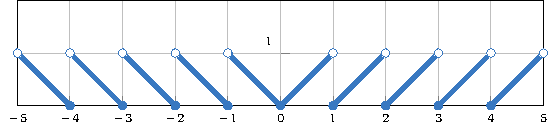
\includepdf[pages=-]{1.pdf}

\cleardoublepage
\phantomsection
\addcontentsline{toc}{chapter}{\numberline{4}Espacios recubridores}

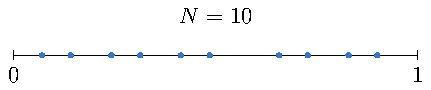
\includepdf[pages=-]{2.pdf}

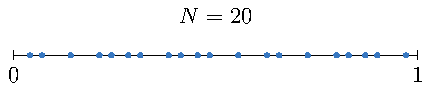
\includepdf[pages=-]{3.pdf}

\end{document}